%! Public Domain Software 2022-2025
%! 2025-08-27
%! 4.0.5-beta
%! Elayson Abreu
%! abntexto.classe@gmail.com

% !TeX TS-program = lualatex
\documentclass{abntexto}

\usepackage[german,english,brazil,shorthands=off]{babel}
\usepackage[cmyk]{xcolor}
\usepackage{lipsum}
\usepackage[
    style       = abnt,
    maxbibnames = 100,
    extrayear   = true,
]{biblatex} \addbibresource{abntexto.bib}
\usepackage{unicode-math}
\usepackage[colorlinks,linktoc=page]{hyperref}
\usepackage{microtype}
\usepackage[brazilian,capitalize,noabbrev]{cleveref}\AtBeginDocument{\def\ref#1{\cref{#1}}}
\usepackage{fontspec}
\usepackage{listings}
\usepackage{lua-widow-control} \clubpenalty=10000\widowpenalty=10000

\makeatletter

% VERBATIM
% ================================================

\def\adef#1{\catcode`#1=13 \begingroup \lccode`\~=`#1\lowercase{\endgroup\def~}}
\def\setverb{\def\do##1{\catcode`##1=12}\dospecials\space}
\def\verbchar#1{%
    \ifx\savedttchar\undefined\else \catcode\savedttchar=\savedttcharc \fi
    \chardef\savedttchar=`#1\relax
    \chardef\savedttcharc=\catcode`#1\relax
    \adef{#1}{\leavevmode\hbox\bgroup\setverbchar\readverb}%
    \bgroup\lccode`\~=`#1\lowercase{\egroup\def\readverb ##1~}{##1\egroup}%
    \catcode`#1=13
}
\def\setverbchar{\setverb
    \adef{ }{\ }%
    \adef{\{}{\bgroup\normalcolor\char`\{}%
    \adef{\}}{\char`\}\egroup}%
    \adef{[}{\bgroup\normalcolor\char`[}%
    \adef{]}{\char`]\egroup}%
    \ttfamily
}

\edef\bslash{\csstring\\}
\def\mytarget#1{\vbox to0pt{\kern-12pt \hypertarget{#1}{}\vss}}
\def\1{`}\def\2{``}
{\catcode`\`=13 \AtBeginDocument{%
    \verbchar{`}%
    \def\^`{\bgroup \docpoint}%
    \def\docpoint#1`{\egroup\leavevmode\edef\tmp{\csstring#1}%
        \expandafter\parsecn \string#1\relax
        \ifcsname \cn s/^\tmp\endcsname \else
            \mytarget{\cn s/^\tmp}\csgdef{\cn s/^\tmp}{}%
        \fi
        \hyperlink{\cn s/\tmp}{\color{blue}\ttfamily\if\cn c\bslash\fi\tmp}%
    }%
    \def\parsecn #1#2\relax {\edef\cn{\if\bslash#1c\else n\fi}}%
    \def\`{\bgroup \mainpoint}%
    \def\mainpoint #1`{\egroup\leavevmode\edef\tmp{\csstring#1}%
        \expandafter\parsecn \string#1\relax
        \ifcsname \cn s/\tmp\endcsname \moremainpoints \else
            \mytarget{\cn s/\tmp}\csgdef{\cn s/\tmp}{}%
        \fi
        \ifcsname \cn s/^\tmp\endcsname
            \hyperlink{\cn s/^\tmp}{\ttfamily\if\cn c\bslash\fi\tmp}\else
            {\color{red}\ttfamily\string#1}%
        \fi
    }%
    \def\moremainpoints{\errmessage{Second main documentation point \if\cn c\bslash\fi\tmp}}
}}

\let\lchevron=<
{\catcode`<=13 \AtBeginDocument{\catcode`<=13
    \def<#1>{\ifhmode\else\expandafter\hbox\fi\bgroup\normalcolor\ttfamily
             $\color{gray}\langle$\/{\rmfamily\itshape #1\/}$\color{gray}\rangle$\egroup}}%
}

\def\type#1{\NoCaseChange{\protect\typeA{#1}}}
\def\typeA#1{\bgroup\normalshape\ttfamily{\escapechar=-1\relax\expandafter}\detokenize{#1}\egroup}
% Precisamos de \m@ne aqui, \m@ne=-1.
\pdfstringdefDisableCommands{%
    \def\type#1{\bgroup\escapechar\m@ne\expandafter\egroup\detokenize{#1}}%
    \let\escapechar=\relax
    \let\m@ne=\relax
}

\definecolor{P}{RGB}{242, 121, 0}   % Primitivas.
\definecolor{C}{RGB}{23, 230, 23}   % Comentários.
\definecolor{B}{RGB}{245, 250, 247} % Fundo.

\lstset{
    language        = [latex]tex,
    basicstyle      = \abntsmall\singlesp\ttfamily,
    texcsstyle      = *\color{P}, % O listings não permite ":"
    commentstyle    = \color{C},  % no nome dessas cores. Bug.
    backgroundcolor = \color{B},
    frame           = leftline,
    rulecolor       = \color{lightgray},
    columns         = fullflexible,
    breaklines      = false,
    keepspaces      = true,
    aboveskip       = 0pt plus1.2ex minus.67ex,
    belowskip       = 0pt plus1.2ex minus.67ex,
    abovecaptionskip = 0pt,
    belowcaptionskip = 0pt,
%    tabsize         = 1, % Sem efeito, porque o documento usa Espaço na tabulação.
}

% #1 = linewidth
% #2 = border
% #3 = padding
% #4 = padding-top
% #5 = padding-right
% #6 = padding-bottom
% #7 = padding-left
% #8 = margin-left
% #9 = margin-right
\def\mylstset#1#2#3#4#5#6#7#8#9{\lstset{
    linewidth          = \dimexpr#1 -#2 -#3 -#5\relax,
    framerule          = \dimexpr#2\relax,
    framesep           = \dimexpr#3\relax,
    xleftmargin        = \dimexpr#2 +#3 +#7 +#8\relax,
    xrightmargin       = \dimexpr#9\relax,
    framextopmargin    = \dimexpr#4\relax,
    framexrightmargin  = \dimexpr#5\relax,
    framexbottommargin = \dimexpr#6\relax,
    framexleftmargin   = \dimexpr#7\relax,
}}
\mylstset{\linewidth}{1pt}{0pt}{0pt}{0pt}{0pt}{0pt}{0pt}{0pt}

\lstnewenvironment{lst}[1][\placepos]{%
    \let\medskipamount=\smallskipamount
    \place[#1]\vbox\bgroup
}{%
    \egroup\endplace
}

\def\hookXP{}
\lstnewenvironment{xp}[1][]{%
    \lstset{
        frame           = leftline,
        basicstyle      = \normalsize\ttfamily\singlesp\vskip-\baselineskip,
        texcsstyle      = \normalcolor,
        commentstyle    = \normalcolor,
        backgroundcolor = \color{white},
        gobble          = 4,
    }%
    \mylstset{\linewidth}{0pt}{0pt}{0pt}{0pt}{0pt}{\parindent}{0pt}{0pt}%
    \expandafter\lstset \expandafter{\hookXP,#1}%
    \endgraf\null
}{}

% ETC.
% ================================================

\setmainfont{XITS}[
    UprightFont    = *-Regular,
    BoldFont       = *-Bold,
    ItalicFont     = *-Italic,
    BoldItalicFont = *-BoldItalic,
    Extension      = .otf
]
\setmathfont{XITSMath-Regular.otf}
\setmonofont{InconsolataN}[
    UprightFont = *-Regular,
    BoldFont    = *-Bold,
    Extension   = .otf
]

\definelegendplace{code}{Código}{loc}
\definelegendplace{output}{Saída}{loo}
\definelegendplace{scr}{\emph{Screenshot}}{loscr}

\Crefname{code}{Código}{Códigos}
\Crefname{output}{Saída}{Saídas}
\Crefname{appendix}{Apêndice}{Apêndices}
\Crefname{codesection}{Seção}{Seções}
\Crefname{codesubsection}{Seção}{Seções}
\Crefname{scr}{\emph{Screenshot}}{\emph{Screenshots}}

\let\over=\@@over
\AtBeginDocument{\def\refname{Referências}} % Removido \^ da definição.
\def\hooksection{}
\def\tocsubsectionfont{\itshape}
\def\subsectionfont   {\itshape}
\AtBeginDocument{\pretocmd\appendix{\clearpage}{}{}}
\pretocmd\annex{\clearpage}{}{}
\def\etex{\leavevmode\hbox{$\varepsilon$-\TeX}}
\def\pdflatex{\leavevmode\hbox{PDF\LaTeX}}
\def\xelatex{\leavevmode\hbox{Xe\LaTeX}}
\def\lualatex{\leavevmode\hbox{Lua\LaTeX}}
\def\me{Elaboração própria.}
\def\bibfont{\raggedright\interlinepenalty=10000\singlesp\bibitemsep=\baselineskip}
\appto\textual{
    \def\@evenhead{\abntsmall \firstmarks0\hfil\thepage}
    \def\@oddhead {\abntsmall \botmarks1\hfil\thepage}
    \def\sectionmark   #1{\marks0{Seção \thesection: \unexpanded{#1}}}
    \def\subsectionmark#1{\marks1{Subseção \thesubsection: \unexpanded{#1}}}
    \preto\@oddhead {\lower4pt\rlap{\vrule width\hsize height.4pt}}
    \preto\@evenhead{\lower4pt\rlap{\vrule width\hsize height.4pt}}
}
\patchcmd{\eletroniclayout}{false}{true}{}{}
\let\onesidelayout=\eletroniclayout
\let\twosidelayout=\eletroniclayout
\hypersetup{
    pdfauthor   = Elayson Abreu,
    pdftitle    = Classe ABNTexto: normas ABNT em LaTeX,
    pdfsubject  = Manual da classe ABNTexto,
    pdfcreator  = LaTeX with abntexto,
    pdfkeywords = ABNTexto. LaTeX. Classe. ABNT,
}
\makeatother



\begin{document}
\leavevmode\vskip1.9in
\begingroup \centering \LARGE\sffamily\bfseries
    Classe ABNTexto\vskip-3pt \Large\itshape\mdseries
    Normas ABNT em {\upshape\LaTeX}\vskip2em \normalfont\large
    Elayson Abreu\vskip-3pt
    \href{mailto:abntexto.classe@gmail.com}%
                {abntexto.classe@gmail.com}\vskip2ex
    \today
\vskip2in\endgroup

\noindent\hfil {\Large\ttfamily 4.0.5-beta}
\newpage

\nonum\notoc\section{Sumário}
\maketoc
\newpage

\section{Introdução}

O `abntexto` é uma classe do \LaTeX\ criada para facilitar a utilização das normas da Associação Brasileira de Normas Técnicas (ABNT) em trabalhos acadêmicos (monografias, dissertações, teses). Ela carrega os recursos necessários para a elaboração de trabalhos nessas normas.

Este \emph{não} é um manual sobre LaTeX (ou TeX, a ferramenta que o constitui) nem tampouco uma descrição detalhada sobre as normas ABNT. Para aprender sobre LaTeX leia \textcite{massago-2022-latex2e-via-exemplos}, em português, ou \textcite{martinsen-2022-latex2e-an-unnoficial}, disponível em inglês, espanhol e francês. Além disso, também se pode ler \textcite{olsak-2012-tex-in-nutshell} e \textcite{eijkhout-1992-tex-by-topic}, disponíveis em inglês, para aprender sobre o sistema \TeX.

Já existe uma classe para aplicação das normas ABNT cujo nome é `abntex2` \cite{araujo-2012-a-classe-abntex2}. Mas, diferente dessa, o `abntexto` não depende do `memoir`, uma classe de código-fonte e manual extensos e que implementa funções as quais, em sua maioria, não são pertinentes a um documento que use as diretrizes da ABNT.

As normas ABNT as quais o `abntexto` se propõe a seguir seguem listadas:

\begin{topics}
    \item NBR 14724:2024. Informação e documentação --- Trabalhos acadêmicos --- Apresentação \cite{abnt-2024-14724-trabalhos-academicos};
%    \item NBR 12225:2004. Informação e documentação --- Lombada --- Apresentação \cite{abnt-2004-12225-lombada};
%    \item NBR 6028:2021. Informação e documentação --- Resumo --- Apresentação \cite{abnt-2021-6028-resumo-resenha-recensao};
    \item NBR 6027:2012. Informação e documentação --- Sumário --- Apresentação \cite{abnt-2012-6027-sumario};
    \item NBR 10520:2023. Informação e documentação --- Citações em documentos --- Apresentação \cite{abnt-2023-10520-citacoes};
%    \item NBR 6023:2018. Informação e documentação --- Referências --- Elaboração \cite{abnt-2018-6023-referencias};
%    \item NBR 5892:2019. Informação e documentação --- Representação e formatos de tempo --- Datas e horas --- Apresentação \cite{abnt-2019-5892-representacao-e-formatos-de-tempo};
    \item NBR 6024:2012. Informação e documentação --- Numeração progressiva das seções de um documento --- Apresentação \cite{abnt-2012-6024-numeracao-progressiva-das};
    \item IBGE. Normas de apresentação tabular \cite{ibge-1993-normas-de-apresentacao}.
\end{topics}

\subsection{Nota de compatibilidade}

No salto da versão anterior, 3.2.1-beta, para esta, 4.0.0-beta, muito do código-fonte foi reescrito; funcionalidades foram adicionadas; comandos obsolesceram. Por consequência, documentos antigos irão certamente quebrar em \emph{layout} e aparência.

Para que os usuários tenham tempo de atualizar para esta nova versão, o arquivo `abntexto-3-2-1-beta.cls` foi deixado no repositório da classe no CTAN\footnote{\url{https://ctan.org/pkg/abntexto}.}. Todavia, para documentos antigos que já foram concluídos, não faz sentido atualizá-los para a versão atual. Nesse caso, seria pertinente copiar o arquivo `abntexto-3-2-1-beta.cls` para o mesmo diretório do documento cuja fase de escrita já foi concluída, chamá-lo por meio de `\documentclass{abntexto-3-2-1-beta}`, e, dessa forma, garantir que o resultado da compilação seja sempre o mesmo.

Para usuários que desejam atualizar seus documentos, o `abntexto` preservou a funcionalidade de comandos obsoletados até onde foi possível e muitas mensagens de alerta/erro foram criadas.

\subsection{Mudanças e novidades}

A sintaxe de `\place{<conteúdo>}` foi substituída por `\begin{place}[<opcional>]`. Além disso, após requisições, a classe ganhou suporte para objetos flutuantes. O posicionamento de `place` pode ser alterado em `<opcional>` com as palavras-chave de objetos flutuantes: `!, t, b, p, h`. Além destas, a classe criou uma nova: `here`\footnote{Semelhante a especificação `H` do pacote `float` \cite{float-package}.}. Com ela, o usuário impõe que `<conteúdo>` seja exibido no PDF na mesma posição em que foi inserido no documento.

Comandos da forma `\<ext>labelwidth` tais como `\toclabelwidth`, `\appendixlabelwidth`, entre outros, não precisam mais ser configurados, porque o `abntexto` alinha os rótulos de suas respectivas entradas automaticamente com a ajuda dos novos comandos `\eqbox` e `\eqboxsize`.

O pacote `enumitem` é carregado pela classe e o ambiente `topics` foi reescrito em função do referido pacote.

A partir de agora, use `\abntsmall` ao invés de `\small`. Por enquanto, o significado deste será igual ao daquele.

\subsection{\emph{Feedback}}

Sugestões, dúvidas, relatos de \emph{bugs} e doações são bem-vindas:\hfil\break {\ttfamily abntexto.classe@gmail.com}.

Chave PIX: {\ttfamily abntexto.classe@gmail.com}

\section{Chamando a classe}

O autor da classe recomenda o uso do \lualatex\ na compilação, embora o \pdflatex\ e o \xelatex\ também sejam suportados. Digite as linhas do \ref{cd:inicio} em conjunto com o \lualatex\ e use `abntexto`.

\legend{code}{Início}
\src\me
\label{cd:inicio}
\begin{lst}
    \documentclass{abntexto}

    \usepackage[english,brazil]{babel}
    \usepackage{fontspec}
    \usepackage{unicode-math}

    \setmainfont{XITS}[
        UprightFont    = *-Regular,
        BoldFont       = *-Bold,
        ItalicFont     = *-Italic,
        BoldItalicFont = *-BoldItalic,
        Extension      = .otf
    ]
    \setmathfont{XITSMath-Regular.otf}

    \begin{document}
        Texto
    \end{document}
\end{lst}

O arquivo `abntexto-exemplo.tex`, disponível no diretório da classe no CTAN, mostra como elaborar os elementos pré-textuais.

\section{Fonte tipográfica}

O tamanho da fonte é 12\,pt de imediato e pode ser configurado redefinindo `\normalsize` por meio de \^`\definesize`, cuja sintaxe é
\begin{xp}
    \definesize\<seletor>{<tamanho de fonte>}{<entrel. simples>}%
                         {<configs. extras>}
\end{xp}
O primeiro argumento é o nome do seletor (`\normalsize`, por exemplo). O segundo argumento é o tamanho da fonte. O terceiro é a entrelinha simples que deve ser selecionada levando em conta o valor do segundo argumento. Por exemplo, uma fonte com tamanho 10\,pt deve ter por volta de 12\,pt de entrelinha simples. O quarto argumento é para ajuste de valores dependentes do tamanho da fonte, por exemplo `\abovedisplayskip` ou `\bigskipamount`.

A classe `article`, na qual se baseia o `abntexto`, fornece os seletores habituais `\tiny`, `\footnotesize`, `\Large` etc. No entanto, esta classe se limitou a redefinir apenas dois: `\normalsize` para o tamanho padrão do texto e \^`\abntsmall` para satisfazer a exigência da \textcite{abnt-2024-14724-trabalhos-academicos} acerca do tamanho menor e uniforme. Até a versão anterior da classe, 3.2.1-beta, o comando `\small` era usado, mas foi substituído por `\abntsmall` para não haver conflito com o significado original de `\small` da classe `article`.

O espaçamento é de 1,5 por padrão e pode ser alterado com os atalhos \^`\singlesp` e \^`\onehalfsp` que alternam para espaçamento simples e de 1,5, respectivamente\footnote{O \type{\\doublesp} está obsoleto.}. A fórmula desses comandos foi atualizada, portanto documentos com versões antigas do `abntexto` terão o \emph{layout} alterado.

Nesta versão, `\spacing` está obsoleto porque esse comando ainda usa a fórmula antiga. Além disso, ele tem uma limitação: só pode ser usado após um seletor de tamanho, porque tais seletores redefinem `\baselineskip` diretamente. Por exemplo, `\abntsmall\spacing{<fator>}` é correto, porém `\spacing{<fator>}\abntsmall` é ineficaz. Essa limitação não existe ao usar os reimplementados `\singlesp` e `\onehalf` de forma que tanto `\singlesp\onehalfsp` quanto `\onehalfsp\singlesp` produzem o mesmo efeito.

\section{\emph{Layout}}

A folha é A4 por padrão e as margens esquerda e direita são de, respectivamente, 3\,cm, 2\,cm para páginas ímpares e de, respectivamente, 2\,cm, 3\,cm para páginas pares. Além disso, as margens superior e inferior têm, nessa ordem, 3\,cm, 2\,cm para todo o documento. Essas margens foram ajustadas com o pacote `geometry`, carregado na classe.

Existem dois comandos que configuram o \emph{layout} da página: \^`\pretextual` e \^`\textual`. O primeiro é iniciado automaticamente durante `\begin{document}`, invoca \^`\onesidelayout` e remove a numeração de página. O segundo, `\textual`, também é executado automaticamente pelo primeiro `\section` numerado, invoca \^`\twosidelayout` e ativa a numeração de página.

O comando `\onesidelayout` configura as páginas para impressão de somente um lado do papel (anverso) ao passo que `\twosidelayout` espelha as margens do documento, habilitando a impressão para os dois lados do papel (anverso e verso).

Os trabalhos acadêmicos podem vir a ser disponiblizados num repositório \emph{online}. Nesse caso, o usuário pode querer reconfigurar as margens de forma a se ter uma leitura mais confortável em dispositivos eletrônicos. Para esse propósito foi criado o comando \^`\eletroniclayout`, apesar dessa configuração não estar prevista na ABNT.

Há duas formas de ativá-lo. A primeira é, no preâmbulo, redefinir `\pretextual` e `\textual` substituindo as instruções `\onesidelayout` e `\twosidelayout` por `\eletroniclayout`. A segunda possibilidade é, também no preâmbulo, redefinir `\onesidelayout` e `\twosidelayout` diretamente conforme \ref{cd:eletroniclayout}. O comando `\eletroniclayout` centraliza o corpo do texto configurando 2,5\,cm nas margens esquerda e direita.

\legend{code}{\emph{Layout} para dispositivos eletrônicos}
\src\me
\label{cd:eletroniclayout}
\begin{lst}
    \documentclass{abntexto}
    \let\onesidelayout=\eletroniclayout
    \let\twosidelayout=\eletroniclayout
    \begin{document}
        texto
    \end{document}
\end{lst}

Outros comandos de estilo de página tais como `\pagestyle`\{{\ttfamily headings, empty, myheadings, plain}\} herdados da classe `article` não fazem sentido no `abntexto`. Ao invés de usá-los, é aconselhável redefinir `\textual`, `\pretextual` ou ambos.

\section{Sumário}

A classe `article` criou o comando `\tableofcontents` para impressão do Sumário, cuja definição será mantida por compatibilidade. No `abntexto`, porém, é recomendado usar \^`\maketoc`, cuja definição é ligeiramente diferente.

Os comandos que configuram a fonte tipográfica das entradas do Sumário são \^`\tocsectionfont`, \^`\tocsubsectionfont` etc. (ver \ref{cd:contents}). O último token nessas definições pode conter parâmetro, por exemplo:
\begin{xp}
    \def\tocsectionfont{\bfseries\MakeUppercase}
    \def\tocparagraphfont{\fbox}
\end{xp}

\legend{code}{Aparência do Sumário}
\src\me
\label{cd:contents}

\begin{lst}
    \documentclass{abntexto}
    \usepackage{xcolor}
    \def \tocsectionfont    {\color{red}\itshape\MakeUppercase}
    \def \tocsubsectionfont {\color{blue}\bfseries}

    \begin{document}
        \nonum\notoc\section{Sumário}
        \maketoc
        \newpage

        \section{Título}
        \subsection{Título}
    \end{document}
\end{lst}

\section{Secionamento}\label{sec:secionamento}

A personalização das macros de seção (\^`\section`, \^`\subsection`, \^`\subsubsection`, \^`\paragraph` e \^`\subparagraph`) é análoga a personalização do Sumário e deve ser feita redefinindo \^`\sectionfont`, \^`\subsectionfont`, \^`\subsubsectionfont`, \^`\paragraphfont` e \^`\subparagraphfont` como exemplificado em \ref{cd:sec} abaixo.

\src\me
\legend{code}{Aparência das seções}
\label{cd:sec}
\begin{lst}
    \documentclass{abntexto}
    \usepackage{xcolor}
    \def \sectionfont       {\color{blue}\scshape}
    \def \subsectionfont    {\color{red}\itshape}
    \def \subsubsectionfont {\color{yellow}\sffamily}

    \begin{document}
        \nonum\notoc\section{Sumário}
        \maketoc

        \section{Texto}
        \subsection{Texto}
        \subsubsection{Texto}
    \end{document}
\end{lst}

Também há como alterar o espaço vertical acima e abaixo das seções redefinindo \^`\abovesection`, \^`\belowsection`. Por exemplo, `\def\abovesubsection{2cm}` insere um espaço de 2\,cm acima de `\subsection`. Se o leitor deseja zerar essas instruções, deve escrever `\def\abovesubsection{0pt}` ao invés de `\def\abovesubsection{}`.

\subsection{O uso de \type{\\chapter} e \type{\\part}}

De acordo com a ABNT: \enquote{[\dots] O trabalho acadêmico não pode ser dividido em capítulos; deve ser organizado em seções [\dots]}.

O usuário pode querer utilizar capítulos no trabalho, apesar de a unidade secional `\section` ser suficiente para um trabalho acadêmico. Para esse propósito, o `abntexto` disponibiliza a instrução \^`\chapter` para a utilização de capítulos no documento, porém não em conformidade com a \textcite{abnt-2024-14724-trabalhos-academicos}, mas no estilo da classe `book`. Para ativá-los é preciso chamar a instrução \^`\usechapters` no preâmbulo.

Também é possível usar \^`\part` em conjunto com o comando \^`\useparts`. Esse útlimo contém `\usechapters` em sua definição, portanto, ao chamar `\useparts`, não se deve chamar `\usechapters` para que este não sobrescreva as definições daquele.

Os níveis secionais `\section` e `\chapter` podem ser prefixados com \^`\nonum` que remove a numeração do título: `\nonum\section`. Os títulos prefixados com `\nonum` serão centralizados \cite{abnt-2024-14724-trabalhos-academicos}. Veja um exemplo de uso em \ref{cd:nonum}.

\legend{code}{Exemplo de título sem numeração e sem ingresso ao Sumário}
\src\me
\label{cd:nonum}

\begin{lst}
    \nonum\notoc\section{Resumo}
    Texto

    \nonum\notoc\section{Sumário}
    \maketoc
\end{lst}

As unidades secionais supracitadas também podem ser prefixadas com \^`\notoc` que instrui o título a não ingressar no Sumário: `\notoc\section`. Além disso, é possível usar ambos os prefixos ao mesmo tempo, conforme mostrado em \ref{cd:nonum}.

O primeiro parágrafo após uma seção é indentado por padrão, dispensando, assim, o uso do pacote `indentfirst`.

Infelizmente, comandos como `\printbibliography`, `\printglossary` e `\printindex` inserem o título internamente. Para que esse título seja exibido corretamente no `abntexto`, é necessário usar o ambiente \^`corrprint`, como demonstrado em \ref{cd:corrprint}.

\legend{code}{Ambiente \type{corrprint}}
\src\me
\label{cd:corrprint}

\begin{lst}
    \begin{corrprint}
        \printbibliography % ou \printglossary, \printindex e semelhantes
    \end{corrprint}
\end{lst}

Existe a possibilidade de o usuário desejar criar um Índice usando o ambiente `theindex` --- embora alternativas automatizadas sejam preferíveis \cite{martinsen-2022-latex2e-an-unnoficial}. Nesse caso, o ambiente `corrprint` funcionará como esperado conforme explicitado em \ref{cd:corrprint-theindex}. O ambiente `corrprint` também pode ser utilizado com o ambiente `thebibliography`, assim como no exemplo com `theindex`.

\legend{code}{Ambientes \type{corrprint} e \type{theindex}}
\src\me
\label{cd:corrprint-theindex}

\begin{lst}
    \begin{corrprint}
        \begin{theindex}
            \item carro, 1
                \subitem árvore, 2
            \indexspace
            \item mar, 3
                \subitem continente, 4
        \end{theindex}
    \end{corrprint}
\end{lst}

\section{Alíneas}

Use o ambiente \^`topics` para criar alíneas. Ele dispõe de dois níveis sendo que o segundo usa um travessão como marcador conforme o exemplo em \ref{cd:topics}. Naturalmente, é permitido usar `\label` após um item.

\legend{code}{Alíneas}
\src\me
\label{cd:topics}

\begin{lst}
    \begin{topics}
        \item \label{al:x} 1
            \begin{topics}
                \item \label{subal:x} x
                \item y
                \item z
            \end{topics}
        \item \label{al:y} 2
        \item 3
    \end{topics}
\end{lst}

\section{Áreas de legenda\label{sec:area-de-legenda}}

Use o ambiente \^`place` para inserir áreas de legenda. Ele substitui integralmente os ambientes `figure` e `table`, bem como o comando `\caption`, não suportados pela classe. Além disso, tem-se \^`\legend`\nobreak`{<tipo>}{<legenda>}` para titular; \^`\src`\nobreak`{<fonte>}` (\emph{source}) para inserir a fonte como mostrado em \ref{cd:place}. Porém, existem condições: `place` deve constar em último lugar e `\label` deve suceder `\legend`.

\legend{code}{Áreas de legenda}
\src\me
\label{cd:place}

\begin{lst}
    \begin{document}
        \legend{figure}{Um título}
        \src{\texttt{www.site.com.br}. Acesso em 01 jan. 2020.}
        \label{fig:teste}
        \begin{place}
            \includegraphics[width=0.4\linewidth]{example-image}
        \end{place}

        Ver \ref{fig:teste}.
    \end{document}
\end{lst}

Além disso, existe a possibilidade de alterar o espaço vertical acima e abaixo de uma área de legenda com `\def`\^`\aboveplace``{<valor>}` e `\def`\^`\belowplace``{<valor>}`. Todavia, tais comandos não têm efeito em objetos flutuantes. Para modificar o espaçamento em `floats` o leitor pode fornecer valores diferentes para `\floatsep`, `\intextsep` e `\textfloatsep`, definidos no LaTeX.

A partir desta versão, o `abntexto` passou a suportar objetos flutuantes. Por exemplo, em
\begin{xp}
    \begin{place}[<especificação>]
\end{xp}
A `<especificação>` é composta pelas palavras-chave habituais: `!`, `t`, `b`, `p`, e `h`. Alternativamente, é possível usar a palavra-chave `here`, definida nesta classe. Com ela, o conteúdo de `place` é mostrado na página exatamente onde foi escrito no documento.

A especificação padrão é `here` caso nenhuma seja explicitamente assumida, mas o usuário pode mudar o padrão digitando, por exemplo, `\def`\nobreak\^`\placepos``{tbp}` no preâmbulo do documento.

\subsection{Criando áreas de legenda}

Até a versão anterior, 3.2.1-beta, o `abntexto` fornecia \^`\definelegendplace` para criação de novos espaços de legenda sob a sintaxe
\begin{xp}
    \definelegendplace{<tipo>}{<nome>}{<ref rótulo>}{<extensão>}
\end{xp}
Nesta versão, no entanto, o terceiro argumento foi excluído em favor do suporte mais extensivo do pacote `cleveref.sty` (não carregado pela classe). Veja o \ref{app:cleveref} para mais detalhes. A partir de agora, a nova sintaxe é
\begin{xp}
    \definelegendplace{<tipo>}{<nome>}{<extensão>}
\end{xp}
Esta classe continuará fornecendo suporte sintático, porém sem funcionalidade, para a versão anterior do referido comando, mas vai exibir uma mensagem de alerta pedindo para que o terceiro argumento seja removido.

Acerca do novo `\definelegendplace`: a instrução
\begin{xp}
    \definelegendplace{diagram}{Diagrama}{lod},
\end{xp}
por exemplo, criará o comando `\makelod` para escrever no documento as entradas do arquivo auxiliar `.lod`. Além disso, o tipo de legenda `diagram` estará disponível para ser usado em `\legend`: `\legend{diagram}{<título>}`.

\subsection{Figuras lado a lado}

O `abntexto` tem suporte nativo para inserção de figuras lado a lado com o ambiente \^`multiplace`. Elas se comportam como caracteres então podemos usar `\hfil` para centralizá-las. Veja o exemplo no \ref{cd:multiplace} e o resultado em \ref{out:result}.

\legend{code}{Figuras lado a lado}
\src\me
\label{cd:multiplace}
\begin{lst}
    \legend{figure}{Duas figuras}
    \src{Elaboração do autor.}

    \begin{multiplace}
        \sublegend{Um título} \label{fig:teste1}
        \subsrc{\texttt{www.site.com.br}. Acesso em 01 jan. 2020.}
        \hfil
        \begin{subplace}[.25\linewidth]
            \includegraphics[width=\linewidth]{example-image-a}
        \end{subplace}
        %
        \sublegend{Outro título} \label{fig:teste2}
        \subsrc{\texttt{www.site.com.br}. Acesso em 01 jan. 2020.}
        \hfil
        \begin{subplace}[.25\linewidth]
            \includegraphics[width=\linewidth]{example-image-b}
        \end{subplace}
    \end{multiplace}

    \parindent=1.5cm Ver \ref{fig:teste1} e \ref{fig:teste2}.
\end{lst}

\legend{output}{Resultado do \ref{cd:multiplace}}
\label{out:result}
\src\me
\begin{place}\vbox\bgroup
    \legend{figure}{Duas figuras}
    \src{Elaboração do autor.}
    %
    \begin{multiplace}
        \sublegend{Um título} \label{fig:teste1}
        \subsrc{\texttt{www.site.com.br}. Acesso em 01 jan. 2020.}
        \hfil
        \begin{subplace}[.25\linewidth]
            \includegraphics[width=\linewidth]{example-image-a}
        \end{subplace}
        %
        \sublegend{Outro título} \label{fig:teste2}
        \subsrc{\texttt{www.site.com.br}. Acesso em 01 jan. 2020.}
        \hfil
        \begin{subplace}[.25\linewidth]
            \includegraphics[width=\linewidth]{example-image-b}
        \end{subplace}
    \end{multiplace}

    \parindent=1.5cm Ver \ref{fig:teste1} e \ref{fig:teste2}.
\egroup\end{place}

Há uma legenda principal impressa com `\legend` e duas sublegendas para cada objeto inseridas com \^`\sublegend`\nobreak`{<título>}`, bem como um par de ambientes \^`subplace`\footnotemark. Além disso, a ordem das instruções é similar àquela aplicada no ambiente `place`: `subplace` deve ser posto após ambos `\sublegend` e \^`\subsrc``{<fonte>}`, e `\label` deve suceder `\legend`.

\footnotetext{A sintaxe \type{\\subplace{<conteúdo>}} está obsoleta. Use `subplace` na forma de ambiente: \type{\\begin{subplace}}.}

Linhas em branco produzem quebra de parágrafo em `multiplace` e, provavelmente, não são desejadas.

Normalmente, espaços em branco depois de `\end{<env>}` são significativos, mas, no caso do ambiente `subplace`, isso não é verdade, porque existe um `\ignorespacesafterend` em sua definição, um comando definido no LaTeX.

Existe, ainda, a possibilidade de um arranjo diferente no `multiplace` usando o parâmetro opcional de `\sublegend`, como se pode ver no \ref{cd:multialt} em conjunto com o resultado em \ref{out:alt}.

\legend{code}{Uso alternativo de \type{multiplace}}
\src{Elaborado pelo autor.}
\label{cd:multialt}
\begin{lst}
    \begin{multiplace}
        \sublegend[table]{Tabela de exemplo} \label{tab1}
        \subsrc{\me}
        \hfil
        \begin{subplace}[.25\linewidth]
            \includegraphics[width=\linewidth]{example-image-a}
        \end{subplace}
        %
        \sublegend[figure]{Título de figura} \label{fig1}
        \subsrc{\me}
        \hfil
        \begin{subplace}[.25\linewidth]
            \includegraphics[width=\linewidth]{example-image-b}
        \end{subplace}
        %
        \sublegend[figure]{Outra figura} \label{fig2}
        \subsrc{\me}
        \vadjust{\kern10pt}\\ \null \hfil
        \begin{subplace}[.25\linewidth]
            \includegraphics[width=\linewidth]{example-image-c}
        \end{subplace}
    \end{multiplace}
\end{lst}

\src{\me}
\begin{place}\vbox\bgroup
\legend{output}{Resultado do \ref{cd:multialt}} \label{out:alt}
\src{Elaborado pelo autor.}
\begin{multiplace}
    \sublegend[table]{Tabela de exemplo} \label{tab1}
    \subsrc{\me}
    \hfil
    \begin{subplace}[.25\linewidth]
        \includegraphics[width=\linewidth]{example-image-a}
    \end{subplace}
    \sublegend[figure]{Título de figura} \label{fig1}
    \subsrc{\me}
    \hfil
    \begin{subplace}[.25\linewidth]
        \includegraphics[width=\linewidth]{example-image-b}
    \end{subplace}
    \sublegend[figure]{Outra figura} \label{fig2}
    \subsrc{\me}
    \vadjust{\kern10pt}\\ \null \hfil
    \begin{subplace}[.25\linewidth]
        \includegraphics[width=\linewidth]{example-image-c}
    \end{subplace}
\end{multiplace}
\egroup\end{place}

A \ref{out:alt} possui a \ref{tab1}, \ref{fig1} e \ref{fig2}.

\subsection{Tabelas que se partem entre páginas}

No momento não existe suporte para legendar tabelas e outras estruturas que se partem entre páginas. Se o leitor tiver de usar `longtable.sty` \cite{longtable-package} ou `tabularray.sty` \cite{tabularray-package} (este último é mais flexível), será preciso legendar estruturas tabulares com as ferramentas fornecidas por esses pacotes.

\section{Formatação de \type{\\cite} e Referências}

O `abntexto` não possui macros para formatação de `\cite` e Referências. Utilize `\usepackage[style=abnt]{biblatex}`.

\section{Citações}

Visando seguir a norma \textcite{abnt-2023-10520-citacoes}, são fornecidos `\enquote` do pacote `csquotes`, carregado pela classe, e \^`\Enquote`. Para inserir aspas duplas em citações diretas, de até três linhas, use `\enquote{<texto>}\cite{<chave>}`. Porém, se tratando de citações diretas, com mais de três linhas, de parágrafo único, alterne para `\Enquote{<texto> \cite{<chave>}.}`.

\section{Apêndice e Anexo}

Com os comandos \^`\appendix` e \^`\annex` você pode inserir apêndices e anexos junto dos indicativos desejados: \enquote{APÊNDICE 1 --- \dots} ou \enquote{ANEXO 1 --- \dots} (ver \ref{cd:appendix}).

\legend{code}{Anexos e apêndices}
\src{\me}
\label{cd:appendix}

\begin{lst}
    \begin{document}
        \appendix{Lorem}
        \appendix{Lipsum}

        \annex{Lorem}
        \annex{Lipsum}
    \end{document}
\end{lst}

Até a versão anterior desta classe, era necessário ajustar a largura dos rótulos no Sumário manualmente redefinindo os comandos \^`\appendixlabelwidth` e \^`\annexlabelwidth`. Todavia, nesta versão, 4.0.0-beta, eles se ajustam automaticamente com o auxílio das novas macroinstruções \^`\eqbox` e \^`\eqboxsize`.

\section{Macros para identificação do documento}

\subsection{Ficha catalográfica}

Para produzir fichas catalográficas foi criado o ambiente \^`indexcard`. Ele sempre esteve disponível na forma `\indexcard{<conteúdo>}`, agora obsoleta, mas nunca foi devidamente documentado neste manual. Eis uma amostra de uso:
\begin{xp}
    \documentclass{abntexto}
    \usepackage{lipsum}
    \usepackage{xcolor}
    \begin{document}
        \def\icardWidth{12.5cm}
        \def\icardHeight{7.5cm}
        \def\icardPadding{1cm}
        \def\icardBorder{2pt}
        \appto\icardFont{\color{magenta}}
        \icardPrintGrid

        \noindent\hfil
        \begin{indexcard}
            \lipsum[1][1-4]
        \end{indexcard}
    \end{document}
\end{xp}
Que produz:

\bgroup
\def\icardWidth{12.5cm}
\def\icardHeight{7.5cm}
\def\icardPadding{1cm}
\def\icardBorder{2pt}
\appto\icardFont{\color{magenta}}
\icardPrintGrid
\noindent\hfil
\begin{indexcard}
    \lipsum[1][1-4]
\end{indexcard}
\egroup

Perceba que a instrução \^`\icardPrintGrid` desenha uma grade de quatro linhas para delimitar os contornos do bloco de texto, no intuito de verificar se ele não ultrapassou as margens internas. A definição original de `\icardFont` é
\begin{xp}
    \def\icardFont{\raggedright\parindent=2em\ttfamily}
\end{xp}

\subsection{Utilitário \type{\\Enter}}

O `abntexto` criou o comando \^`\Enter``[<número>]` para produzir um espaço vertical equivalente à tecla `Enter` do teclado. Ele é usado com frequência em `abntexto-exemplo.tex`. O argumento opcional `<número>` é o número de `Enters` que será impresso, por exemplo, `\Enter[2]` imprime um espaço vertical equivalente a dois `Enters` consecutivos. Como `\Enter` é, basicamente, `\vskip\baselineskip`, precedê-lo com `\par` não é necessário, porque `\vskip` possui, a grosso modo, um `\par` em seu funcionamento.

\subsection{Desativando a hifenização}

O comando \^`\nohyph` impede a hifenização dos parágrafos integralmente, sendo útil em títulos e parágrafos curtos. Seu uso pode ser feito assim:
\begin{xp}
    {\nohyph Parágrafo curto ou título\par} % Esse \par é necessário para
                                            % que a formatação do parágrafo
                                            % entre em ação.
\end{xp}

\subsection{Assinatura da banca}

Use \^`\judgeline``{<arg>}` para assinaturas na Folha de Aprovação. Exemplo:
\begin{xp}
    \judgeline{Prof. Dr. Nome Sobrenome \\ Instituição}\Enter
    \judgeline{Prof. Dr. Nome Sobrenome \\ Instituição}\Enter
    \judgeline{Prof. Dr. Nome Sobrenome \\ Instituição}
\end{xp}
Resultado:
\judgeline{Prof. Dr. Nome Sobrenome \\ Instituição}\Enter
\judgeline{Prof. Dr. Nome Sobrenome \\ Instituição}\Enter
\judgeline{Prof. Dr. Nome Sobrenome \\ Instituição}

Veja outro exemplo de `\judgeline` em `abntexto-exemplo.tex`.

\newpage
\begin{corrprint}
    \printbibliography
\end{corrprint}

\newrefsection

\appendix{Cleveref\label{app:cleveref}}

Até a versão passada, 3.2.1-beta, o `abntexto` tinha o poder de inferir o tipo de `\ref` e inserir o substantivo correspondente com auxílio do terceiro parâmetro de `\definelegendplace`. No entanto, esse parâmetro foi removido deixando o referido comando com três argumentos apenas. Como resgatar essa funcionalidade de inferência em `\ref`? Usando o pacote `cleveref.sty` e sua macro `\cref` \cite{cleveref-package}. Veja o exemplo em \ref{cd:cleveref}, cujo resultado é \enquote{Ler Seção 1}.

\legend{code}{Exemplo de uso do \type{cleveref.sty}}
\src\me
\label{cd:cleveref}
\begin{lst}
    \documentclass{abntexto}
    \usepackage[brazil]{babel}
    \usepackage[brazilian,capitalize,noabbrev]{cleveref}
    \begin{document}
        \section{Um título de exemplo\label{sec:ex}}
        Ler \cref{sec:ex}.
    \end{document}
\end{lst}

Percebe-se que a chave `brazil` não é reconhecida pelo `cleveref` compelindo-nos a usar `brazilian`. Além disso, ele deve ser carregado depois do `hyperref.sty`. Veja outras funcionalidades no manual do pacote.

\appendix{Lista de Abreviaturas}

Elemento opcional. O `glossaries-extra.sty` \cite{glossaries-extra-package} consegue criar uma Lista de Abreviaturas, conforme \ref{cd:abbrev}.

\legend{code}{Abreviaturas}
\src\me
\label{cd:abbrev}

\begin{lst}
    \documentclass{abntexto}

    \usepackage[brazil]{babel}
    \usepackage{hyperref}
    \usepackage[automake,shortcuts=all,abbreviations]{glossaries-extra}\makeglossaries
    \usepackage[brazilian,capitalize,noabbrev]{cleveref}

    \newabbreviation[category=abbreviations]{fil}{Fil.}{Filosofia}
    \newabbreviation[category=abbreviations]{el sf}{el.\,sf.}{elemento substantivo feminino}
    \newabbreviation[category=abbreviations]{eng el}{Eng.\,Elétr.}{Engenharia Elétrica}
    \newabbreviation[category=abbreviations]{med legal}{Med.\,Leg.}{Medicina Legal}

    \begin{document}
        Abreviaturas: \ab{fil},
                      \ab{el sf},
                      \ab{eng el},
                      \ab{med legal}.

        \begin{corrprint}\notoc % "Lista de Abreviaturas" não deve constar no Sumário.
            \printglossary[type=abbreviations]
        \end{corrprint}
    \end{document}
\end{lst}

Note que o `cleveref.sty` deve ser carregado depois de `glossaries-extra.sty`, e o `hyperref.sty`, antes.

\appendix{Lista de Siglas}

Elemento opcional. O `glossaries-extra.sty` \cite{glossaries-extra-package} também consegue criar uma Lista de Siglas, conforme \ref{cd:acro}.

\legend{code}{Siglas}
\src\me
\label{cd:acro}

\begin{lst}
    \documentclass{abntexto}

    \usepackage[brazil]{babel}
    \usepackage{hyperref}
    \usepackage[automake,shortcuts=all,acronym]{glossaries-extra}\makeglossaries
    \usepackage[brazilian,capitalize,noabbrev]{cleveref}

    \setabbreviationstyle[acronym]{long-short}

    \newacronym{ibge}{IBGE}{Instituto Brasileiro de Geografia e Estatística}
    \newacronym{html}{HTML}{HyperText Markup Language}
    \newacronym{ce}{CE}{Ceará}
    \newacronym{edo}{EDO}{Equação Diferencial Ordinária}

    \begin{document}
        1ª chamada: \ac{ibge}, \ac{html}, \ac{ce}, \ac{edo}.

        2ª chamada: \ac{ibge}, \ac{html}, \ac{ce}, \ac{edo}.

        \begin{corrprint}\notoc % "Lista de Siglas" não deve constar no Sumário.
            \printglossary[type=acronym]
        \end{corrprint}
    \end{document}
\end{lst}

Note que o `cleveref.sty` deve ser carregado depois de `glossaries-extra.sty`, e o `hyperref.sty`, antes.

\appendix{Lista de Símbolos}

Elemento opcional. O `glossaries-extra.sty` \cite{glossaries-extra-package} também consegue criar uma Lista de Símbolos, conforme \ref{cd:simbolos}.

\legend{code}{Símbolos}
\src\me
\label{cd:simbolos}

\begin{lst}
    \documentclass{abntexto}

    \usepackage[brazil]{babel}
    \usepackage{hyperref}
    \usepackage[automake,shortcuts=all,symbols]{glossaries-extra}\makeglossaries
    \usepackage[brazilian,capitalize,noabbrev]{cleveref}

    \def\newsymbol#1#2#3#4{\newglossaryentry{#1}{
        name={#2},sort={#3},description={#4},type=symbols,category=symbol}}

    \newsymbol{alpha}{\ensuremath{\alpha}}{a}{Letra grega alfa}
    \newsymbol{o(n)}{\ensuremath{O(n)}}{On}{Ordem de um algoritmo}
    \newsymbol{i}{\ensuremath{i}}{i}{Unidade imaginária}
    \newsymbol{A}{\ensuremath{\mathbf{A}}}{A}{Matriz $\mathbf{A}$}
    \newsymbol{N}{N}{N}{Newton}

    \def\symb#1{\gls{#1}}

    \begin{document}
        Símbolos: \symb{alpha}, \symb{o(n)}, \symb{i}, \symb{A}, \symb{N}.

        \begin{corrprint}\notoc % "Lista de Símbolos" não deve constar no Sumário.
            \printglossary[type=symbols]
        \end{corrprint}
    \end{document}
\end{lst}

Note que o `cleveref.sty` deve ser carregado depois de `glossaries-extra.sty`, e o `hyperref.sty`, antes.

\appendix{Glossário}

Elemento opcional. Você pode criar glossários com `glossaries-extra` \cite{glossaries-extra-package}, como em \ref{cd:gloss}.

\legend{code}{Glossário}
\src\me
\label{cd:gloss}

\begin{lst}
    \documentclass{abntexto}

    \usepackage[brazil]{babel}
    \usepackage{hyperref}
    \usepackage[automake,shortcuts=all]{glossaries-extra}\makeglossaries
    \usepackage[brazilian,capitalize,noabbrev]{cleveref}

    \newglossaryentry{metalismo}{
        name        = metalismo,
        description = {Tipo de sistema monetário cujo valor da moeda,
                       geralmente de uma nação ou de um país, é determinado
                       pela quantidade constante de certo metal (ouro ou
                       prata), desta forma se estabelece um valor fixo de
                       troca entre esses metais e o próprio dinheiro.}
    }
    \newglossaryentry{backend}{
        name        = \emph{backend},
        sort        = backend,
        description = {A parte de um site ou aplicação que não é visível
                       para o usuário e que gerencia a lógica de negócios
                       e a comunicação com o banco de dados.}
    }
    \newglossaryentry{cache}{
        name        = cache,
        description = {Um armazenamento temporário de dados para acesso
                       rápido. Ajuda a reduzir o tempo de carregamento.}
    }
    \newglossaryentry{autovetor}{
        name        = autovetor,
        description = {Um vetor não nulo que, quando multiplicado por uma
                       matriz, resulta em um vetor que é um múltiplo escalar do
                       vetor original.}
    }

    \begin{document}
        Glossário: \gls{metalismo}, \gls{backend}, \gls{cache}, \gls{autovetor}.

        \begin{corrprint}
            \printglossary[type=main]
        \end{corrprint}
    \end{document}
\end{lst}

Note que o `cleveref.sty` deve ser carregado depois de `glossaries-extra.sty`, e o `hyperref.sty`, antes.

% MACROS PARA O CÓDIGO-FONTE
% ================================================

\pdfstringdefDisableCommands{\def\marks#1#2{}}
\appendix{\marks0{}\marks1{}Código-fonte\label{ap:codigo-fonte}}

\makeatletter
\newcounter{codesection}
\newcounter{codesubsection}[codesection]
\let\c@section=\c@codesection
\let\c@subsection=\c@codesubsection
\def\thecodesection{\arabic{codesection}}
\def\thecodesubsection{\thecodesection.\arabic{codesubsection}}
\edef\toclevel@codesection{\mainseclevel}
\edef\toclevel@codesubsection{\the\numexpr\mainseclevel-1\relax}

\appto\hooktocsection{\def\extleaders{}%
    \edef\savedskips{\rightskip=\the\rightskip \parfillskip=\the\parfillskip\relax}}
\appto\hooktocsubsection{\def\extleaders{}%
    \edef\savedskips{\rightskip=\the\rightskip \parfillskip=\the\parfillskip\relax}}
\appto\hookextline{\savedskips}

\def\toclabelbox{\lowercase{\eqbox{codetoc}}}
\def\tocsectionfont{\itshape\MakeUppercase}
\def\tocsubsectionfont{}
\def\sectionfont{\tocsectionfont}
\def\subsectionfont{\itshape}

% O \addcontentsline{#1}{#2}{#3} está programado para
% enviar marcadores apenas se #1 = toc. Podemos
% mudar isso com \hypersetup{bookmarkstype=<outro>}.
\hypersetup{bookmarkstype=codetoc}
\patchcmd{\targetsection}{\refstepcounter{section}}{\refstepcounter{codesection}}{}{}
\patchcmd{\targetsection}{\addcontentsline{toc}}{\addcontentsline{codetoc}}{}{}
\patchcmd{\targetsubsection}{\refstepcounter{subsection}}{\refstepcounter{codesubsection}}{}{}
\patchcmd{\targetsubsection}{\addcontentsline{toc}}{\addcontentsline{codetoc}}{}{}

\def\hooksection{}
\def\codesection{\section}
\def\codesubsection{\subsection}

\colorlet{C}{.}
\definecolor{tmp}{RGB}{128, 0, 32}    \colorlet{P}{tmp}
\definecolor{tmp}{RGB}{255, 228, 236} \colorlet{B}{tmp}

\expanded{\noexpand\lstdefinelanguage{mylang}{
    language    = [latex]tex,
    texcs       = {\directlua{for k,v in pairs(tex.primitives())
                   do tex.print(k, v.. ',')end}},
    deletetexcs = {end}
}}

\lstset{
    language    = mylang,
    frame       = single,
    numbers     = left,
    numbersep   = \dimexpr-5pt+\addnumbersep\relax,
    numberstyle = \fontsize{8bp}{9bp}\selectfont,
    literate    = {\^^M\%.}{}1,
}
\def\addnumbersep{9pt}
\mylstset{\linewidth}{0pt}{0pt}{3pt}{0pt}{3pt}{13pt+\addnumbersep}{0pt}{0pt}

\newcount\codecount \codecount=1
\newbox\mybox
\setbox\mybox=\hbox to\hsize{\hfil\abntsmall\ttfamily\bfseries\color{gray}abntexto.cls}
\lstnewenvironment{code}[1][]{%
    \lstset{
        title       = \copy\mybox\nobreak,
        firstnumber = \codecount,
        #1
    }%
}{%
    \global\codecount=\value{lstnumber}\relax
}
\appto\hookXP{
    frame     = none,
    numbers   = none,
    numbersep = 0pt,
    gobble    = 4,
}

\parskip=0pt plus.2ex minus.1ex
\@starttoc{codetoc}
{\def\excl{!}\catcode\1\!=14 \catcode\1\%=9 %! Public Domain Software 2022-2025
%! 2025-08-27
%! 4.0.5-beta
%! Elayson Abreu
%! abntexto.classe@gmail.com

% \codesection{RECOMENDAÇÕES\label{codesec:rec}}

% Macros internas não devem ser modificadas ou usadas direta ou indiretamente no
% documento. Isso porque essas macros podem ser redefinidas ou até renomeadas em
% futuras versões desta classe. Por macros internas entende-se aquelas com o
% prefixo do pacote em questão, neste caso, `tnba@`. Se você precisa de algum
% comando interno, defina outro sem anexar o prefixo.

% Redefinir arquivos `.sty`, `.cls`, entre outros, diretamente no diretório da
% sua distribuição TeX também não é aconselhado, pelo mesmo motivo exposto no
% parágrafo anterior.

% Copiar arquivos `.sty`, `.cls` etc. para o mesmo diretório do seu documento e
% modificá-los pode ser útil. Nesse caso, é preciso renomeá-los após as
% alterações para não haver confusão em relação ao original (principalmente se o
% arquivo alterado for compartilhado).

% \codesection{ESTILO DE CÓDIGO}

% O formato Plain \TeX\ define atalhos como `\chardef\@ne=1` e `\chardef\tw@=2`
% que, na época em que foi concebido, nos anos 80, serviam para diminuir o tempo
% de compilação\footnote{\url{https://tex.stackexchange.com/questions/9787/ne-tw-thr}.}.
% Para fins semelhantes, \LaTeX\ define `\def\hb@xt@{\hbox to}`,
% `\def\@height{height}` e outros mais. Com a eficiência computacional atual,
% todavia, esses atalhos só são úteis em situações onde se queira a máxima
% performance. Sendo assim, no `abntexto`, esses atalhos serão deixados de lado
% em favor da legibilidade de código.

% Além disso, arrobas (@) serão evitados de modo geral a fim de reduzir a
% necessidade do uso de `\makeatletter` e `\makeatother` em documentos.

% \codesection{INICIALIZAÇÃO}

% Identificação do formato \TeX\ e da classe.

% \begin{code}
\NeedsTeXFormat{LaTeX2e}

\ProvidesClass{abntexto}%
    [2025-08-27 4.0.5-beta Preparation of works in ABNT standards]
%. \end{code}

% Estas são as únicas dependências do `abntexto`. Os pacotes `enumitem` e
% `etoolbox` foram adicionados nesta versão (4.0.x-beta). O primeiro permite
% personalizar listas usando interfaces \emph{key-value}. O segundo oferece
% macros úteis como `\appto` e `\csletcs` para programadores de macros.

% \begin{code}
\LoadClass{article}

\RequirePackage{geometry}
\RequirePackage{graphicx}
\RequirePackage[autostyle=true]{csquotes}
\RequirePackage{enumitem}
\RequirePackage{etoolbox}
%. \end{code}

% Atalhos para `\ClassWarning` e `\ClassError`.

% \begin{code}
\def\tnba@warning#1{\ClassWarning{abntexto}{#1.}}
\def\tnba@error#1{\ClassError{abntexto}{#1}{}}
%. \end{code}

% Os comandos `\pdfbookmark` e `\phantomsection` pertencem ao `hyperref.sty`.
% Infelizmente, no entanto, o `\pdfbookmark` insere um destino de \emph{link}
% sem altura, por isso teremos de parametrizar `\Hy@writebookmark` por
% meio de `\makeoutline`.

% Parametrizaremos `\NR@gettitle` para suporte ao `nameref.sty`, por meio de
% `\processsectitle`. Infelizmente, o comando \NR@gettitle não tem versão
% não-prefixada. A instrução `\processsectitle` expande para `\NR@gettitle` caso
% o pacote `nameref` esteja carregado. Do contrário, `\processsectitle` está
% programado para absorver o argumento. A instrução `\NR@gettitle`, de fato,
% configura `\@currentlabelname` para ser usado em `\nameref`.

% \begin{code}
\AtBeginDocument{%
    \@ifpackageloaded{hyperref}{%
        \def\makeoutline#1#2#3{\Hy@writebookmark{#2}{#3}{\@currentHref}{#1}{toc}}%
    }{%
        \def\makeoutline#1#2#3{}%
        \def\phantomsection{}%
    }%
    \@ifpackageloaded{nameref}{%
        \def\processsectitle#1{\NR@gettitle{#1}}%
    }{%
        \def\processsectitle#1{}%
    }%
}
%. \end{code}

% O `hyperref.sty` verifica se `\pdfstringdefPreHook` existe. Se sim, ele é
% usado, senão um novo é criado. Essa âncora servirá para desativar comandos que
% devem expandir de forma diferente nas linhas da Lista de Marcadores do PDF.

% \begin{code}
\def\pdfstringdefPreHook{}
%. \end{code}

% \codesection{A MACRO \type{\\eqbox}}

% A macro \`\eqbox` foi adaptada de OpTeX e foi introduzida nesta versão do
% `abntexto` (4.0.x-beta). São caixas que, ao receberem um mesmo rótulo, vão se
% igualar com a largura da maior caixa após duas compilações \cite{optex}.
% Exemplo de uso:

% \leavevmode
% \hbox{\begin{xp}[boxpos=t]
%   \noindent
%   \eqbox{x}{ab}?\\
%   \eqbox{x}{abc}?\\
%   \eqbox{x}{abcd}?
%. \end{xp}}\quad
% \hbox{\vtop{
%   \noindent
%   \eqbox{x}{ab}?\\
%   \eqbox{x}{abc}?\\
%   \eqbox{x}{abcd}?
% }}
% \par\nointerlineskip\vbox{}

% Elas serão úteis para definir a largura dos rótulos do Sumário, Listas de
% Siglas, Abreviaturas, Símbolos, Figuras e estruturas semelhantes. Do
% contrário, o usuário final precisaria pôr valores para `\toclabelwidth`,
% `\appendixlabelwidth`, `\annexlabelwidth`, entre outros, para que, assim, após
% 10 ou 15 compilações manuais, alcançar um valor próximo do exato. Se a fonte
% ou tamanho de fonte forem alterados, mais compilações seriam necessárias.

% Diferente da versão em OpTeX, a `\eqbox` nesta classe foi modificada para ter
% uma sintaxe LaTeX-amigável: `\eqbox[<alinhamento horizontal>]{<rótulo>}{<texto>}`.
% Os valores para o parâmetro opcional são `l`, `c` ou `r`. Se o parâmetro
% opcional não for chamado, `l` é usado como padrão \cite{optex}.

% Na primeira compilação, a instrução `\eqbox` anexa
% `\Xeqbox{<rótulo>}{<largura>}` no arquivo auxilar `.aux` e as caixas são
% imprimidas na forma que estão. Já na segunda compilaçao, `\begin{document}`
% chama `\input{\jobname.aux}` e cada ocorrência de
% `\Xeqbox{<rótulo>}{<largura>}` entra em ação. A aparência das caixas no
% arquivo `.aux` é semelhante a exemplificada a seguir:
% \begin{xp}
%   \Xeqbox{<rótulo>}{5.8769pt}
%   \Xeqbox{<rótulo>}{8.2784pt}
%   \Xeqbox{<rótulo>}{12.877pt}
%. \end{xp}

% O arquivo `.aux` é chamado entre `\begingroup` e `\endgroup`, exigindo que
% prefixemos `\global` em `\csdef` para que o valor `\tnba@eqb@<rótulo>` se
% torne conhecido.

% Por fim, o valor da maior largura de uma caixa de determinado rótulo é
% acessível por meio de \`\eqboxsize`\nobreak`{<rótulo>}{<valor>}`, também foi
% copiada do formato OpTeX \cite{optex}. Na primeira compilação, `\eqboxsize`
% utiliza <valor> como largura. Essa macro é expansível em contextos de expansão
% completa (dentro de `\edef`, por exemplo).

% O `\eqbox` terá o \emph{status} `\protected` para não ser expandido por
% `\MakeUppercase`.

% \begin{code}
\def\Xeqbox#1#2{%
    \ifcsname tnba@eqb@#1\endcsname
        \ifdim #2>\csname tnba@eqb@#1\endcsname\relax \global\csdef{tnba@eqb@#1}{#2}\fi
    \else \global\csdef{tnba@eqb@#1}{#2}\fi
}
\protected\def\eqbox{\@ifnextchar[\starteqbox{\starteqbox[l]}}

\def\starteqbox[#1]#2#3{\setbox0=\hbox{{#3}}%
    \immediate\write\@auxout {\string\Xeqbox{#2}{\the\wd0}}%
    \ifcsname tnba@eqb@#2\endcsname
        \hbox to\csname tnba@eqb@#2\endcsname{%
             \ifcsname starteqbox#1\endcsname \csname starteqbox#1\endcsname\relax
             \else \tnba@warning{Parâmetro opcional "#1" desconhecido em "\string\eqbox".
                                 Use "l", "r" ou "c"}\starteqboxl
             \fi
        }%
    \else \tnba@obs@eqbox \box0 \fi
}
\def\starteqboxl{\unhbox0\hss}
\def\starteqboxr{\hss\unhbox0}
\def\starteqboxc{\hss\unhbox0\hss}

\def\tnba@obs@eqbox{\tnba@warning{Recompile para o cálculo da \string\eqbox}%
    \global\let\tnba@obs@eqbox=\relax
}

\appto\pdfstringdefPreHook{%
    \def\eqbox#1#2{#2}%
}

\def\eqboxsize#1#2{\ifcsname tnba@eqb@#1\endcsname\csname tnba@eqb@#1\endcsname\else#2\fi}
%. \end{code}

% \codesection{FONTE TIPOGRÁFICA}

% O tamanho 12\,pt foi definido usando \`\definesize` e é o tamanho padrão da
% classe. Com ele foi definido um tamanho menor \`\abntsmall`.

% Para configurar um tamanho de fonte para o documento, precisamos definir
% `\normalsize` por meio de
% \begin{xp}
%   \definesize\<seletor>{<tamanho>}%
%                        {<entrelinha simples>}{<instruções extras>}
%. \end{xp}
% A seguir, um documento exemplificando seu uso:
% \begin{xp}
%   \documentclass{abntexto}
%   \usepackage{lmodern}
%   \definesize\normalsize{17pt}{20pt}{}
%   \begin{document}
%       Texto lorem lipsum dolor
%   \end{document}
%. \end{xp}
% O exemplo acima já produz efeito sobre o tamanho de fonte, porque o LaTeX
% inicializa `\normalsize` durante `\begin{document}`.

% \codesubsection{O ponto \TeX\ \emph{versus} o ponto DTP}

% Quando \TeX\ foi criado, a unidade ponto (pt) valia $1\over72,27$ de polegada
% pelo Sistema de Ponto Americano. Donald Knuth adotou esse padrão. Nos anos que
% seguiram, com o advento da impressão digital, o ponto passou a ser aceito como
% $1\over72$ de polegada. Esse ponto é conhecido como Desktop Publishing Point,
% PostScript Point ou CSS Point. Felizmente, \TeX\ tem suporte para o ponto DTP
% através da unidade \enquote{bp} (\emph{big point})\footnotemark. Vamos usá-la
% na definição da entrelinha e tamanho de fonte nos seletores do `abntexto`.

% \bgroup
% \def\UrlBreaks{\do\-}
% \footnotetext{\url{https://tex.stackexchange.com/questions/200934/why-does-a-tex-point-differ-from-a-desktop-publishing-point}.}
% \egroup

% \codesubsection{Definindo conjuntos de tamanho de fonte}

% Até a versão anterior do `abntexto` (3.2.1-beta), o comando `\small` era usado
% para selecionar o tamanho menor e uniforme conforme a ABNT NBR 10\,520:
% \Enquote{Recomenda-se, quando digitado, a fonte tamanho 12 para todo o
% trabalho, inclusive capa, excetuando-se citações com mais de três linhas,
% notas de rodapé, paginação, dados internacionais de catalogação-na-publicação,
% legendas e fontes das ilustrações e das tabelas, que devem ser em
% \textit{tamanho menor e uniforme} \cite[p.~10, grifo
% próprio]{abnt-2024-14724-trabalhos-academicos}.} Nesta versão, 4.0.x-beta, ele
% será renomeado para `\abntsmall`, de forma a não haver confusão com o
% significado original do comando `\small` da classe `article`. Por enquanto, o
% significado de `\small` será igual ao de `\abntsmall` para compatibilidade com
% documentos antigos.

% O `\setamounts` configura `\<value>amount`s conforme o tamannho de fonte.

% \begin{code}
\def\hooknormalsize{\setamounts}
\def\hookabntsmall{\setamounts}
\def\setamounts{%
    \dimen4=\f@size pt
    \bigskipamount=\dimen4 plus.33333\dimen4 minus.33333\dimen4
    \medskipamount=.5\dimen4 plus.16666\dimen4 minus.16666\dimen4
    \smallskipamount=.25\dimen4 plus.08333\dimen4 minus.08333\dimen4
}
\input{size12.clo}
\def\definesize#1#2#3#4{\DeclareRobustCommand#1{\@setfontsize{#1}{#2}{#3}#4\relax}}
\definesize\normalsize{12bp}{13.8bp}{\hooknormalsize} % 13.8 = 12 * 1.15
\definesize\abntsmall{10bp}{11.5bp}{\hookabntsmall} % 11.5 = 10 * 1.15
\def\small{\abntsmall} % Para compatibilidade com versões anteriores da classe.
\normalsize
%. \end{code}

% \codesubsection{Espaçamento simples e de 1,5 do Microsoft Word}

% Até a versão anterior (3.2.1-beta), o `abntexto` utilizava a fórmula
% $$
%    `\baselineskip` = <tamanho de fonte> * <fator espaçamento>
% $$
% para o cálculo do espaçamento simples e de 1,5, onde o <tamanho de fonte> é
% dado em pontos. Nela, se o fator espaçamento simples for de 1,2 e o tamanho da
% fonte for de 12~pt, teremos o valor $`\baselineskip` = 12 * 1,2 = 14,4$~pt
% para a entrelinha simples. No entanto, quando a
% \textcite{abnt-2024-14724-trabalhos-academicos} menciona as expressões
% \enquote{espaçamento simples} e \enquote{espaçamento 1,5}, ela deve estar
% referindo-se às fórmulas wordianas desses conceitos, exigindo uma análise mais
% aprofundada sobre eles: \Enquote{Todo texto deve ser digitado ou datilografado
% com espaçamento 1,5 entre as linhas, excetuando-se as citações de mais de três
% linhas, notas de rodapé, referências, legendas das ilustrações e das tabelas,
% natureza (tipo do trabalho, objetivo, nome da instituição a que é submetido e
% área de concentração), que devem ser digitados ou datilografados em espaço
% simples. As referências, ao final do trabalho, devem ser separadas entre si
% por um espaço simples em branco
% \cite[][p.~10]{abnt-2024-14724-trabalhos-academicos}.}

% Segundo a Microsoft\footnotemark, o espaçamento simples é um pouco menor que o
% espaçamento 1,15 e o espaçamento 1,5 é um pouco menor que o espaçamento 2.
% Todavia, isso não clarifica-nos acerca da real definição de espaçamento do
% Word.

% \footnotetext{Extraído da URL: \url{https://www.microsoft.com/en-us/microsoft-365-life-hacks/writing/single-spacing-vs-double-spacing}.}

% Por enquanto, deixaremos o Word em segundo plano e falaremos sobre outro
% programa de processamento de texto: Adobe InDesign. De acordo com o
% ex-cientista principal da Adobe, Dov Isaacs, a fórmula usada no programa Adobe
% InDesign é\footnote{Extraído da URL:
% \url{https://community.adobe.com/t5/indesign-discussions/line-spacing-in-indesign/m-p/11586306?profile.language=pt}.}:
% $$
%    `\baselineskip` = <tamanho> * <fator simples> * <fator espaçamento>
% $$
% A qual é, de fato, equivalente a:
% $$
%    `\baselineskip` = <entrel. simples> * <fator espaçamento> \eqno (1)
% $$
% Como consequência, pode-se afirmar que espaçamento simples é sinônimo de
% espaçamento 1. Partindo do ponto de que essa fórmula é a mesma do Word,
% teremos de
% \begin{topics}
%    \item Abrir o Word\footnote{Versão testada: Office LTSC Professional Plus 2024 - Volume License; Word versão 2048.};
%    \item Remover espaços obtusos conforme \ref{scr:zere};
%          \legend{scr}{Zerando espaços verticais extras}
%          \src{\me}
%          \label{scr:zere}
%          \begin{place}
%             \fbox{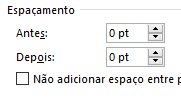
\includegraphics{screenshot1.png}}
%          \end{place}
%    \item Aplicar o espaçamento 1,5 e salvar o arquivo em PDF sob o nome `onehalf-word.pdf`.
% \end{topics}

% Em seguida, ao realizar testes empíricos com auxílio do \ref{cd:emp}, o valor
% <entrelinha> foi incrementado até chegar-se num valor visivelmente próximo ao
% exibido no Word, constatando-se que o espaçamento 1,5 vale $<entrelinha> =
% 20,7\hbox{pt}$.

% \legend{code}{Procedimentos empíricos no Plain LuaTeX}
% \src{\me}
% \label{cd:emp}
% \begin{place}
% \begin{xp}[basicstyle=\abntsmall\ttfamily\singlesp]
%   \input luaotfload.sty
%   \font\times="Times New Roman" at12bp \times
%   \baselineskip=<entrelinha> % Valor 20,7pt descoberto.
%   \noindent
%   Lorem ipsum dolor\hfil\break
%   Lorem ipsum dolor\hfil\break
%   Lorem ipsum dolor\hfil\break
%   Lorem ipsum dolor
%   \bye
%. \end{xp}
% \end{place}

% Logo depois, foi feita a divisão $20,7\hbox{pt} \div 12\hbox{pt} \div
% 1,5\hbox{pt}$ que revela 1,15 como sendo o fator simples. Em seguida, o
% arquivo foi compilado e salvo sob o nome `onehalf-tex.pdf`. Todavia, não
% podemos garantir que esse fator, ou a fórmula em questão, são os mesmos em
% todas as versões passadas/futuras do Word e tampouco os mesmos em todos os
% tipos e tamanhos de fonte.

% Para fins de comparação, foi compilado o \ref{cd:comparacao-no-lualatex},
% exibido na \ref{output:tex-word}.

% \legend{code}{Comparação no LuaLaTeX}
% \src{\me}
% \label{cd:comparacao-no-lualatex}
% \begin{place}
% \begin{xp}[basicstyle=\abntsmall\ttfamily\singlesp]
%   \documentclass{abntexto}
%   \begin{document}
%   \baselineskip=20.7bp
%   \def\.{\kern20.7bp \kern-.4pt % Correção da largura da linha de base.
%          \hrule width8cm height.4pt}
%   \vbox to0pt{\kern-6bp \.\.\.\.\vss}
%   \fbox{\vbox to3cm{\hsize=3.5cm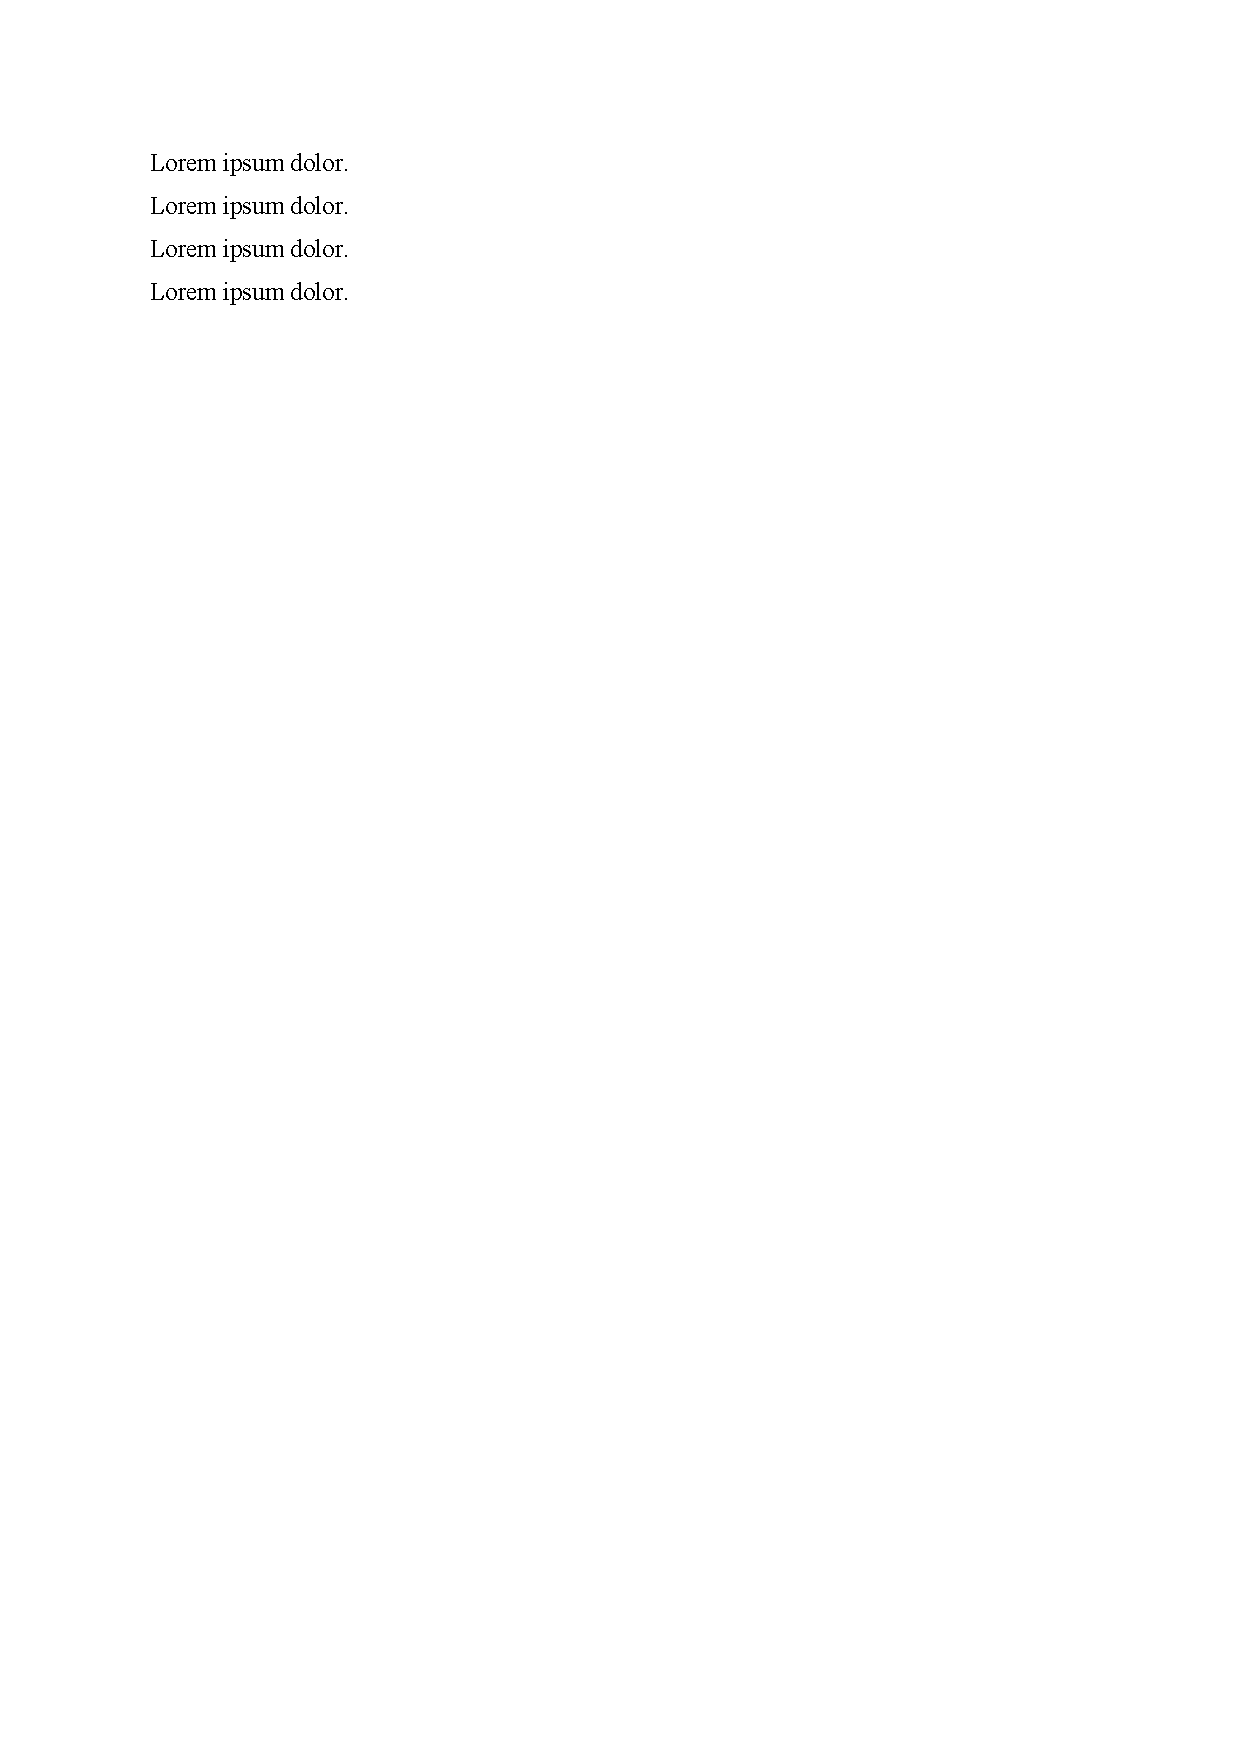
\includegraphics[trim=70 690 420 72]{onehalf-tex.pdf}\vss}}%
%   \fbox{\vbox to3cm{\hsize=3.5cm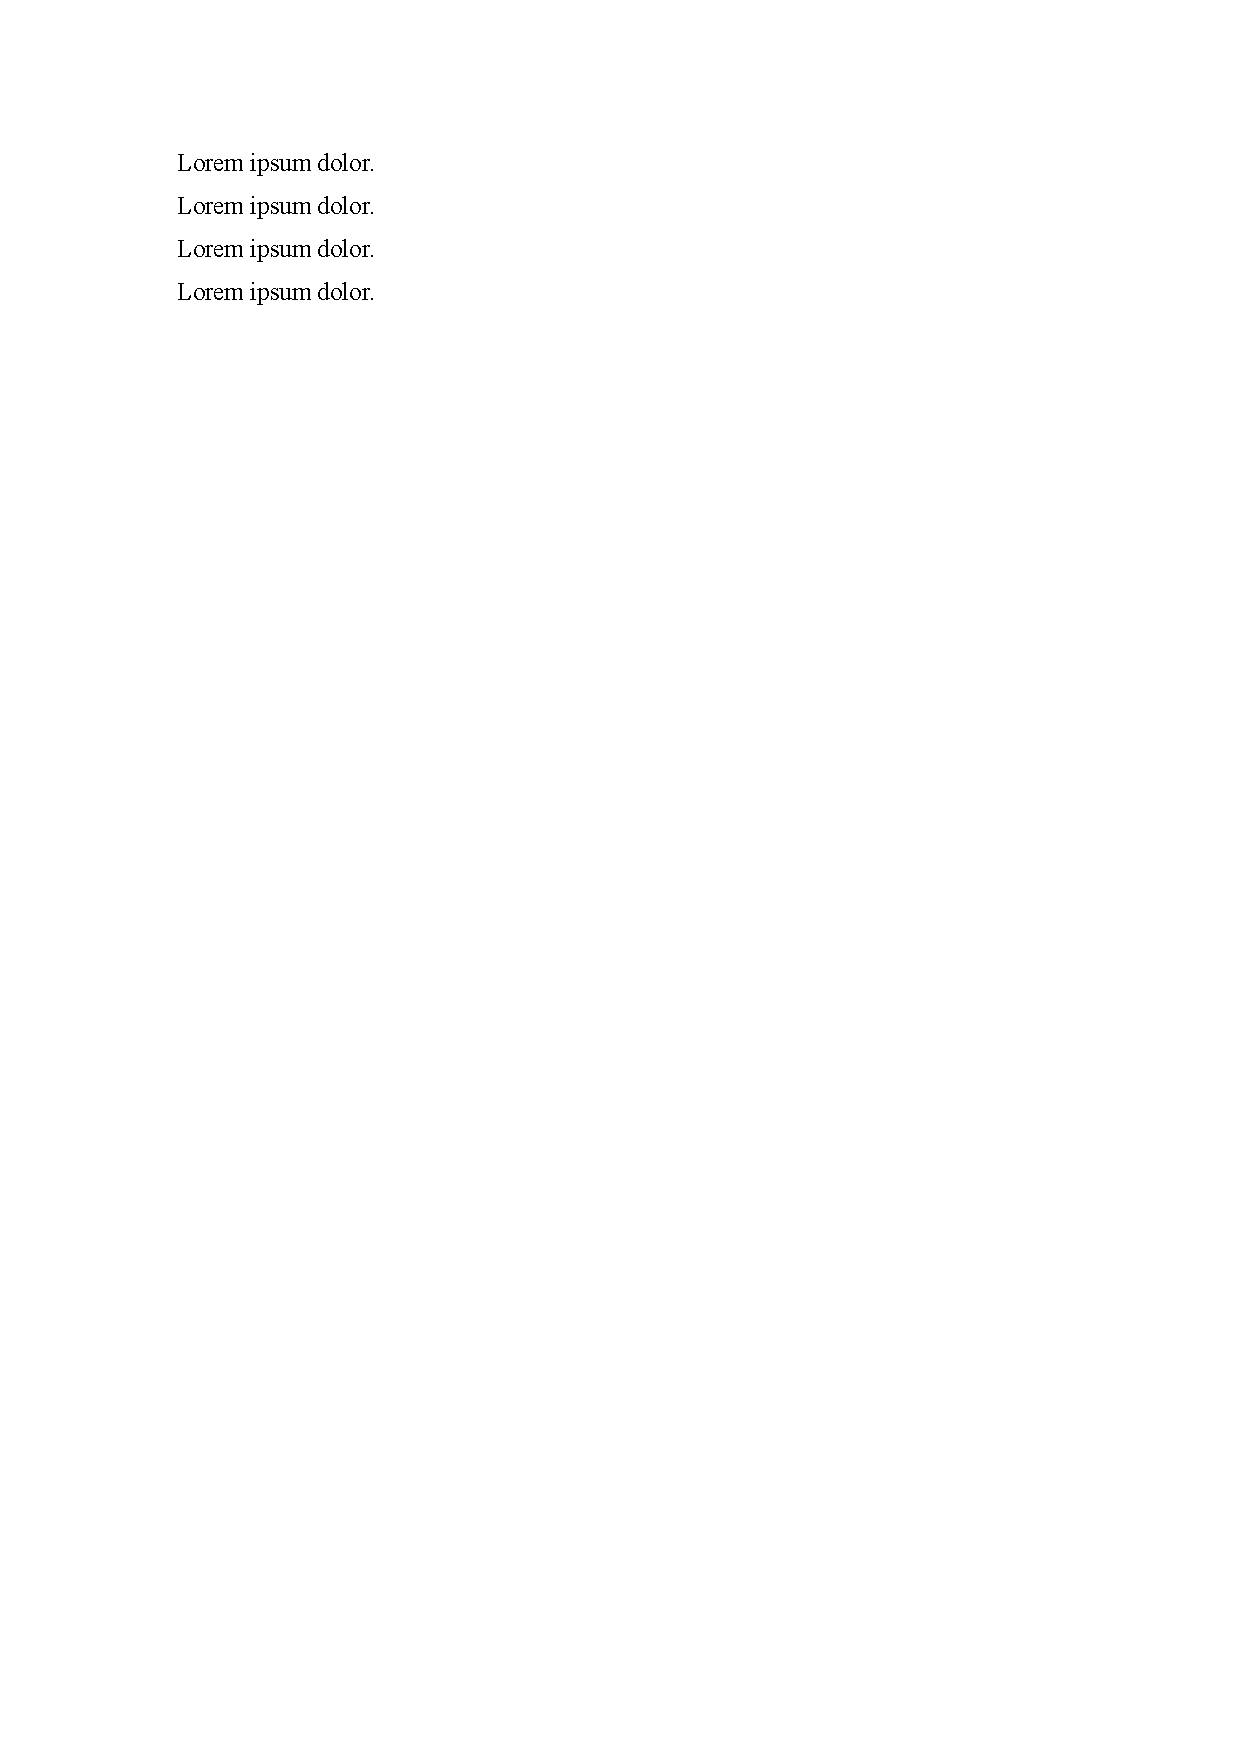
\includegraphics[trim=83 690 420 72]{onehalf-word.pdf}\vss}}
%   \end{document}
%. \end{xp}
% \end{place}

% \legend{output}{Arquivo \type{onehalf-tex.pdf} à esquerda; \type{onehalf-word.pdf} à direita}
% \src{\me}
% \label{output:tex-word}
% \begin{place}\vbox\bgroup\hsize=7.5cm
%   \baselineskip=20.7bp
%   \def\.{\kern20.7bp \kern-.4pt
%          \hrule width8cm height.4pt}
%   \vbox to0pt{\kern-6bp \.\.\.\.\vss}
%   \fbox{\vbox to3cm{\hsize=3.5cm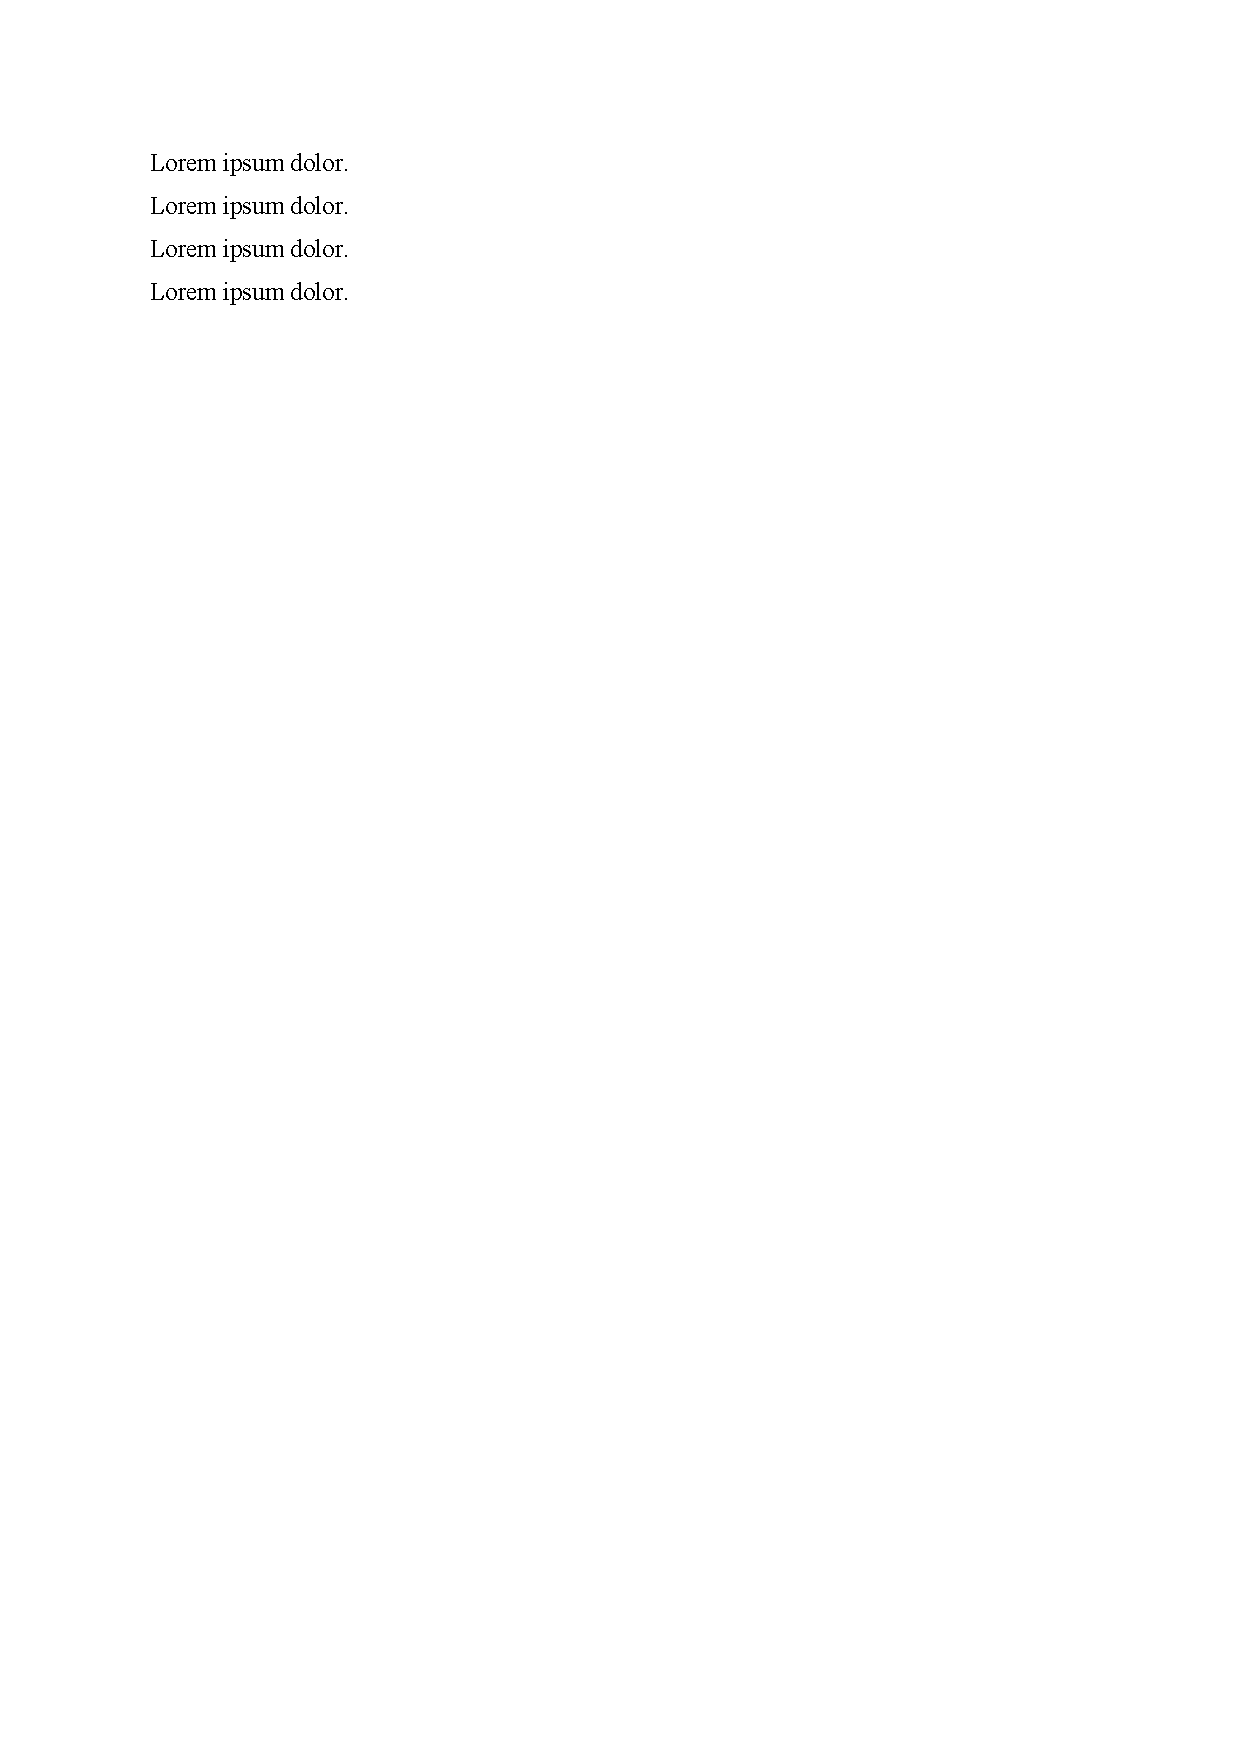
\includegraphics[trim=70 690 420 72]{onehalf-tex.pdf}\vss}}%
%   \fbox{\vbox to3cm{\hsize=3.5cm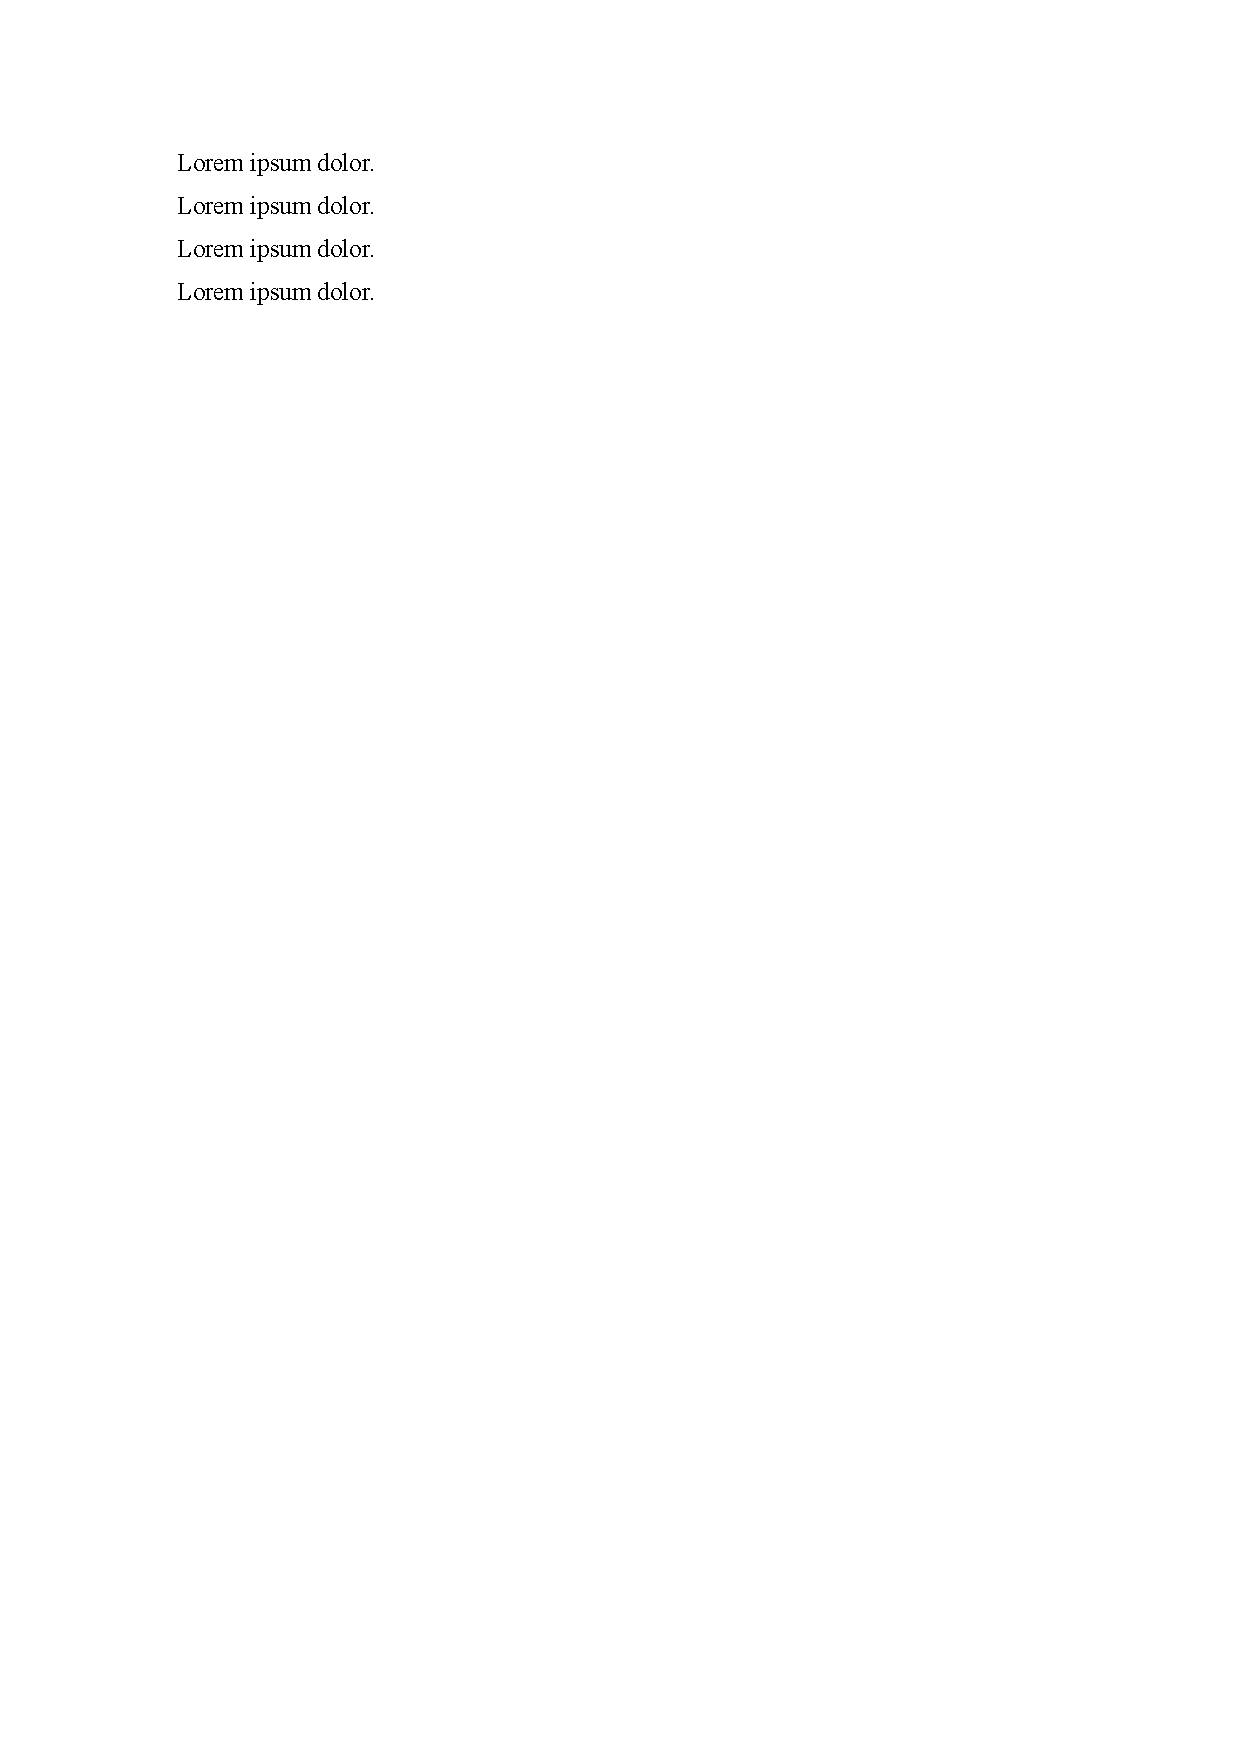
\includegraphics[trim=83 690 420 72]{onehalf-word.pdf}\vss}}
% \egroup
% \end{place}

% O comando `\linespread{<fator espaçamento>}` é exatamente o que precisamos
% para implementar a fórmula~(1) nos espaçamentos simples e de 1,5. Tomemos o
% exemplo:
% \begin{xp}
%   \normalsize\linespread{1.5}\selectfont
%. \end{xp}
% Ele expande, em essência, para `\set@fontsize`\footnote{Não confundir com \type{\\@setfontsize} que também existe.}:
% \begin{xp}
%   \fontsize{12pt}{13.8pt}\selectfont
%   \set@fontsize{1.5}{\f@size}{\f@baselineskip}\selectfont
%. \end{xp}
% As macros `\f@size` e `\f@baselineskip` expandem para o tamanho de fonte atual
% em~`pt` (sem a unidade) e a entrelinha simples atual em~`pt` (com a unidade).
% Dessa forma, teremos, em essência:
% \begin{xp}
%   \fontsize{12pt}{13.8pt}\selectfont
%   \set@fontsize{1.5}{12}{13.8pt}\selectfont
%. \end{xp}
% Finalmente, após mais uma etapa de expansão, obteremos, em essência:
% \begin{xp}
%   \fontsize{12pt}{13.8pt}\selectfont
%   \baselineskip=13.8pt \baselineskip=1.5\baselineskip
%. \end{xp}
% Onde o tamanho de fonte 12~pt permaneceu inalterado e a entrelinha foi configurada para
% $$
%   `\baselineskip` = \hbox{13.8~pt} * 1.5 \eqno \hbox{\vrule width1.5ex height1.5ex}
% $$
% Que corresponde à aplicação da fórmula~(1).

% A \textcite{abnt-2024-14724-trabalhos-academicos} não recomenda espaçamento
% duplo em nenhum momento. Portanto, `\doublesp` está obsoleto a partir desta
% versão do `abntexto`. Por fim, a antiga fórmula usada por `\spacing` também
% está obsoleta.

% O \`\singlesp` e o \`\onehalfsp` iniciam os espaçamentos simples e de 1,5,
% respectivamente.

% \begin{code}
\def\singlesp{\linespread{1}\selectfont}
\def\onehalfsp{\linespread{1.5}\selectfont}
\def\doublesp{\tnba@obsolete\doublesp{}\linespread{2}\selectfont}

\def\spacing#1{%
    \tnba@obsolete\spacing{Use "\string\singlesp" ou "\string\onehalfsp", ao invés}%
    \baselineskip=\f@size pt
    \baselineskip=#1\baselineskip
    \ignorespaces
}
%. \end{code}

% \codesection{\emph{LAYOUT}}

% Nas linhas abaixo estão as definições de \`\onesidelayout`, \`\twosidelayout`
% e \`\eletroniclayout`.

% É importante notar que, cada chamada de `\newgeometry`, reseta, de `\geometry`
% e `\usepackage`, os valores anteriores de chaves não relacionadas com o
% tamanho da folha tais como `left`, `top`, `right` e `bottom`, entre outras
% exigindo que sejam reafirmadas em cada chamada de `\newgeometry`\footnote{Além
% disso, \type{\\newgeometry} também reseta as opções do \type{\\newgeometry}
% anterior, apesar disso não estar explicitado no manual.}.

% Este manual erroneamente afirmava que `\newgeometry` resetava `\parindent`.

% \begin{code}
\geometry{a4paper,onecolumn}

\def\onesidelayout{%
    \newgeometry{
        twoside = false,
        left    = 3cm,
        top     = 3cm,
        right   = 2cm,
        bottom  = 2cm
    }%
}
\def\twosidelayout{%
    \newgeometry{
        twoside = true,
        left    = 3cm,
        top     = 3cm,
        right   = 2cm,
        bottom  = 2cm
    }%
}
\def\eletroniclayout{%
    \newgeometry{
        twoside = false,
        left    = 2.5cm,
        top     = 3cm,
        right   = 2.5cm,
        bottom  = 2cm
    }%
}
%. \end{code}

% Os estilos de página \`\pretextual` e \`\textual` são definidos aqui.

% \begin{code}
\frenchspacing
\onehalfsp
\parskip=0pt
\parindent=1.5cm
\emergencystretch=2em

\def\pretextual{%
    \onesidelayout
    \let\@oddhead=\empty
    \let\@evenhead=\empty
    \let\@oddfoot=\empty
    \let\@evenfoot=\empty
}
\def\textual{%
    \twosidelayout
    \def\@oddhead{\hfil\abntsmall\thepage}%
    \def\@evenhead{\abntsmall\thepage\hfil}%
    \let\@oddfoot=\empty
    \let\@evenfoot=\empty
}
%. \end{code}

% O `\pretextual` é iniciado automaticamente pela classe, mas não diretamente,
% caso o usuário queira redefiní-lo no preâmbulo.

% \begin{code}
\AtBeginDocument{\pretextual}
%. \end{code}

% A \textcite{abnt-2024-14724-trabalhos-academicos} diz que \enquote{para
% trabalhos digitados ou datilografados somente no anverso, todas as folhas, a
% partir da folha de rosto, devem ser contadas sequencialmente, considerando
% somente o anverso. [\dots]}. Todavia, o `abntexto` ainda não tem suporte
% automático para esse requisito.

% \codesection{SUMÁRIO\label{codesec:sumario}}

% O \`\tocsectionfont`, \`\tocsubsectionfont` e semelhantes foram definidos aqui. A macro `\extline` foi baseada em `\@dottedtocline`, definida no LaTeX
% \cite{source2e}. Uma âncora de abstração de nome `\hookextline` foi deixada em
% `\extline` para permitir que o escritor insira parâmetros de ajuste de
% parágrafo, do tipo:

% \begin{xp}
%   \def\hookextline{\emergencystretch=2.5em\hbadness=10000\relax}
%. \end{xp}

% A macro `\noprotrusion` foi definida no LaTeX e serve para desabilidar
% protrusão (\emph{\selectlanguage{english}hanging punctuation}) em entradas do
% Sumário, que pode ser produzida, por exemplo, pelo `microtype.sty`. Se a sua
% versão do LaTeX não o possui, defina-o:

% \begin{xp}
%   \def\noprotrusion{\leavevmode\kern-1pt\kern1pt}
%. \end{xp}

% \begin{code}
\def\tocpartfont          {\bfseries\MakeUppercase}
\def\tocchapterfont       {\bfseries\MakeUppercase}
\def\tocsectionfont       {\bfseries\MakeUppercase}
\def\tocsubsectionfont    {\bfseries\itshape}
\def\tocsubsubsectionfont {\itshape}
\def\tocparagraphfont     {}
\def\tocsubparagraphfont  {}

\def\hookextline{}
\def\extpagenumwidth{1.55em} % \@pnumwidth em article.cls
\def\extrightmargin{2.55em}  % \@tocrmarg em article.cls

% #1 = recuo de parágrafo
% #2 = largura do rótulo
% #3 = fonte tipográfica
% #4 = título
% #5 = número de página
\def\extline#1#2#3#4#5{%
    \begingroup
        \parindent=0pt \leftskip=#1\relax
        \rightskip=\extrightmargin\relax \parfillskip=-\rightskip
        \advance\leftskip by#2\relax
        \hookextline \hskip-#2\relax #3{#4}%
        \extleaders \nobreak\hbox to\extpagenumwidth{\hfil #5\noprotrusion}%
    \nbpar\endgroup
}
%. \end{code}

% O valor `\tocbigvalue` é o espaço vertical que precede as entradas do tipo
% `\part`; `\tocmedvalue`, o valor que precede seções e capítulos;
% `\tocsmallvalue`, o valor para as entradas restantes.

% Não existe preenchimento pontilhado entre título e número de página em
% entradas geradas com `\section`, a não ser que `\usechapters` ou `\useparts`
% esteja ativo. De qualquer forma, o preenchimento pontilhado em seções pode ser
% habilitado assim:

% \begin{xp}
%   \appto\hooktocsection{\let\extleaders=\extdotleaders}
% \end{xp}

% A penalidade $-300$ foi retirada de `\@secpenalty` \cite{source2e}.

% \begin{code}
\def\tocbigvalue{1.576em plus1pt} % 2.25em plus1pt em article.cls
\def\tocmedvalue{.7004em plus1pt} % 1em plus1pt em article.cls
\def\tocsmallvalue{0pt plus.2pt}  % article.cls

\def\l@part         #1#2{{\hooktocpart
                          \extline{0pt}\toclabelwidth\tocpartfont{#1}{#2}}}
\def\l@chapter      #1#2{{\hooktocchapter
                          \extline{0pt}\toclabelwidth\tocchapterfont{#1}{#2}}}
\def\l@section      #1#2{{\hooktocsection
                          \extline{0pt}\toclabelwidth\tocsectionfont{#1}{#2}}}
\def\l@subsection   #1#2{{\hooktocsubsection
                          \extline{0pt}\toclabelwidth\tocsubsectionfont{#1}{#2}}}
\def\l@subsubsection#1#2{{\hooktocsubsubsection
                          \extline{0pt}\toclabelwidth\tocsubsubsectionfont{#1}{#2}}}
\def\l@paragraph    #1#2{{\hooktocparagraph
                          \extline{0pt}\toclabelwidth\tocparagraphfont{#1}{#2}}}
\def\l@subparagraph #1#2{{\hooktocsubparagraph
                          \extline{0pt}\toclabelwidth\tocsubparagraphfont{#1}{#2}}}
%. \end{code}

% O `\tocfirst` serve para remover material vertical (penalidades, colas
% verticais etc.) que não pode ser impresso na primeira entrada do Sumário para
% que não haja espaço duplicado após `\nonum\notoc\section{Sumário}`. Ele
% absorve seu argumento na primeira expansão e redefine a si mesmo para
% `\let\tocfirst=\@firstofone`.

% \begin{code}
\def\hooktocpart   {\tocfirst{\penalty-300\vskip\tocbigvalue}\def\extleaders{\nobreak\hfil}}
\def\hooktocchapter{\tocfirst{\penalty-300\vskip\tocmedvalue}\def\extleaders{\nobreak\hfil}}
\def\hooktocsection{\tocfirst{\penalty-300\vskip\tocmedvalue}\def\extleaders{\nobreak\hfil}}
\def\hooktocsubsection   {\vskip\tocsmallvalue\relax}
\def\hooktocsubsubsection{\vskip\tocsmallvalue\relax}
\def\hooktocparagraph    {\vskip\tocsmallvalue\relax}
\def\hooktocsubparagraph {\vskip\tocsmallvalue\relax}

\def\tocfirst#1{\gdef\tocfirst##1{##1}}

\def\extdotleaders{\nobreak
    \leaders\hbox{$\mathsurround=0pt\mkern4.5mu\hbox{.}\mkern4.5mu$}\hfil
}
\let\extleaders=\extdotleaders
%. \end{code}

% A definição de `\toclabelbox` necessita do `\lowercase` a fim de proteger o
% segundo argumento de `\eqbox` contra `\MakeUppercase` em situações como

% \begin{xp}
%   \def\tocsectionfont{\MakeUppercase}
% \end{xp}

% A diretiva \`\maketoc` é análoga a instrução `\tableofcontents`, definida em
% `article.cls`; o `\@starttoc` (definido no LaTeX) pode ser usado não apenas
% para criar sumários, mas também listas em geral, como Listas de Figuras,
% Tabelas etc. as quais são armazenadas em arquivos de extensão predefinida, a
% saber, `.toc`, `.lof`, `.lot`, entre outros.

% O `\tocfirst` precisa ser restaurado ao fim de `\@starttoc` no caso deste ter
% mais de uma ocorrência no documento.

% \begin{code}
\def\toclabelwidth{\eqboxsize{toc}{2em}}
\def\toclabelbox{\lowercase{\eqbox{toc}}}
\def\toclabel#1{#1\quad}

\appto\pdfstringdefPreHook{%
    \def\quad{\space}%
}

\def\inittocfirst{\gdef\tocfirst##1{\gdef\tocfirst####1{####1}}}
\def\maketoc{\@starttoc{toc}\inittocfirst}
\def\tableofcontents{\nonum\notoc\csname\mainsecname\endcsname{\contentsname
    \@mkboth{\MakeUppercase\contentsname}{\MakeUppercase\contentsname}}%
    \@starttoc{toc}\inittocfirst
} % Para compatibilidade com a classe article.
%. \end{code}

% \codesection{SECIONAMENTO}

% Nesta parte estão definidos os comandos secionais \`\sectionfont`,
% \`\subsectionfont`, \`\subsubsectionfont`, \`\paragraphfont` e
% \`\subparagraphfont` assim como \`\abovesection`, \`\belowsection` e
% similares. Eles podem ser redefinidos pelo usuário.

% \begin{code}
\newcounter{chapter}

\def\sectionfont       {\bfseries\MakeUppercase}
\def\subsectionfont    {\bfseries\itshape}
\def\subsubsectionfont {\itshape}
\def\paragraphfont     {}
\def\subparagraphfont  {}

\def\abovechapter       {50pt}
\def\abovesection       {\baselineskip}
\def\abovesubsection    {\baselineskip}
\def\abovesubsubsection {\baselineskip}
\def\aboveparagraph     {\baselineskip}
\def\abovesubparagraph  {\baselineskip}

\def\belowchapter       {40pt}
\def\belowsection       {\baselineskip}
\def\belowsubsection    {\baselineskip}
\def\belowsubsubsection {\baselineskip}
\def\belowparagraph     {\baselineskip}
\def\belowsubparagraph  {\baselineskip}

\def\thepart          {\Roman{part}}
\def\thechapter       {\arabic{chapter}}
\def\thesection       {\arabic{section}}
\def\thesubsection    {\thesection .\arabic{subsection}}
\def\thesubsubsection {\thesubsection .\arabic{subsubsection}}
\def\theparagraph     {\thesubsubsection .\arabic{paragraph}}
\def\thesubparagraph  {\theparagraph .\arabic{subparagraph}}
%. \end{code}

% As âncoras `\hookprintchapter` e `\hookprintsection` serão usadas na definição
% de `\appendix` e `\annex`.

% O comando `\@hangfrom` é oriundo de `source2e.pdf` \cite{source2e}. Ele vai
% ser útil na formatação das seções.

% A macro `\nbpar` (\emph{no break par}) impede que um parágrafo se quebre entre
% páginas. A instrução `\endgraf` em sua definição, é um comando do `plain.tex`
% definido como `\let\endgraf=\par`. Sua função é guardar o significado original
% de `\par` para situações onde este possa ser redefinido.

% \begin{code}
\def\hookprintchapter{}
\def\hookprintsection{}

\let\hangfrom=\@hangfrom
\def\nbpar{{\interlinepenalty=10000\endgraf}}
%. \end{code}

% Os comandos `\toptitle` e `\bottitle` foram inspirados em `\abovetitle` e
% `\belowtitle` do OpTeX \cite{optex}. Aqueles tem o mesmo funcionamento dos
% originais, explicitado nos casos abaixo:

% \begin{topics}
%   \item $`\nobreak\bottitle{<skipA>}` + `\toptitle{<penaltyA>}{<skipB>}`$
%         $$\offinterlineskip\halign{$#$\cr
%           `\nobreak\vskip<skipB>`;
%         \cr}$$
%   \item $<skipA> + `\toptitle{<penaltyB>}{<skipB>}`$
%         $$\offinterlineskip\halign{$#$\cr
%           <penaltyB>`\vskip` \mathop{\fam0 maior} (<skipA>, <skipB>).
%         \cr}$$
% \end{topics}

% \begin{code}
\newskip \savedtitleskip
\newskip \savedlastskip

\def\toptitle #1#2{\savedlastskip=\lastskip
    \ifdim\lastskip>0pt \vskip-\lastskip \fi
    \ifnum\lastpenalty=11333 \vskip-\savedtitleskip \else #1\fi
    \ifdim\savedlastskip>0pt \setbox0=\vbox{#2\global\dimen3=\lastskip}%
    \else \dimen3=\maxdimen \fi
    \ifdim\savedlastskip>\dimen3 \vskip\savedlastskip \else #2\relax \fi
}
\def\bottitle #1{#1\global\savedtitleskip=\lastskip \penalty11333 }
%. \end{code}

% As próximas linhas definem o \emph{layout} dos comandos de seção, sendo que os
% \emph{designs} de `\printchapter` e `\printpart` não foram baseados no estilo
% ABNT, mas copiados das classes `book` e `article`, respectivamente.

% A \textcite{abnt-2024-14724-trabalhos-academicos} recomenda que haja um
% caractere de Espaço entre o contador e o título das seções. No entanto, esta
% classe optou pelo uso de `\quad`, mas o escritor pode redefinir
% `\printsection` substituindo `\quad` por Espaço usando o comando `\patchcmd`
% do `etoolbox.sty` da seguinte forma:

% \begin{xp}
%   \patchcmd{\printsection}{\quad}{\space}{}{}
%   \patchcmd{\printsubsection}{\quad}{\space}{}{}
%   ...
% \end{xp}

% \begin{code}
\def\printpart#1{\hookpart \leavevmode\vfil
    \noindent\targetpart{#1}%
    \begingroup
        \centering\huge\bfseries Parte \thepart \vskip20pt
        \Huge\bfseries #1\par
    \endgroup \newpage
}
\def\printchapter#1{\hookchapter \trytextual
    \leavevmode \vskip\abovechapter\relax
    \noindent\targetchapter{#1}%
    \begingroup
        \raggedright\huge\bfseries
        \ifnonum \else Capítulo \thechapter \vskip20pt \fi
        \Huge\bfseries \hookprintchapter{#1\par}%
    \endgroup
    \chaptermark{#1}%
    \nobreak \bottitle{\vskip\belowchapter}%
}
\def\printsection#1{\hooksection \trytextual
    \par\toptitle{\penalty-300}{\vskip\abovesection}%
    \noindent\targetsection{#1}%
    \ifnonum
        {\centering\sectionfont{\hookprintsection{#1\nbpar}}}%
    \else
        {\sectionfont{\hangfrom{\thesection\quad}#1\nbpar}}\sectionmark{#1}%
    \fi
    \nobreak \bottitle{\vskip\belowsection}%
}
\def\printsubsection#1{\par\toptitle{\penalty-300}{\vskip\abovesubsection}%
    \noindent\targetsubsection{#1}%
    {\subsectionfont{\hangfrom{\thesubsection\quad}#1\nbpar}}\subsectionmark{#1}%
    \nobreak \bottitle{\vskip\belowsubsection}%
}
\def\printsubsubsection#1{\par\toptitle{\penalty-300}{\vskip\abovesubsubsection}%
    \noindent\targetsubsubsection{#1}%
    {\subsubsectionfont{\hangfrom{\thesubsubsection\quad}#1\nbpar}}%
    \nobreak \bottitle{\vskip\belowsubsubsection}%
}
\def\printparagraph#1{\par\toptitle{\penalty-300}{\vskip\aboveparagraph}%
    \noindent\targetparagraph{#1}%
    {\paragraphfont{\hangfrom{\theparagraph\quad}#1\nbpar}}%
    \nobreak \bottitle{\vskip\belowparagraph}%
}
\def\printsubparagraph#1{\par\toptitle{\penalty-300}{\vskip\abovesubparagraph}%
    \noindent\targetsubparagraph{#1}%
    {\subparagraphfont{\hangfrom{\thesubparagraph\quad}#1\nbpar}}%
    \nobreak \bottitle{\vskip\belowsubparagraph}%
}
%. \end{code}

% Aqui estão \`\nonum` e \`\notoc`. Os comandos secionais `\part`, `\chapter` e `\section` têm âncoras em suas definições que servem para instruções de quebra de página.

% \begin{code}
\def\hookpart{\clearpage}
\def\hookchapter{\clearpage}
\def\hooksection{\clearpage}

\newif\ifnotoc
\newif\ifnonum

\def\nonum{\global\nonumtrue}
\def\notoc{\global\notoctrue}
\def\resetnonumnotoc{\global\notocfalse \global\nonumfalse}
%. \end{code}

% As diretivas da forma `\target<name>` são, em essência, definidas assim:
% \begin{xp}
%   \def\target<nome>#1{%
%       \refstepcounter{<contador>}%
%       \addcontentsline{<ext>}{<seção>}{#1}}
%. \end{xp}
% O `\refstepcounter` avança o <contador> e cria um destino de \emph{hyperlink}.
% Já `\addcontentsline`, escreve `#1` num comando da forma `\l@<seção>` e
% imprime o resultado no arquivo de extensão <ext>. Se o `hyperref.sty` for
% chamado, `\addcontentsline` adicionalmente cria uma entrada na Lista de
% Marcadores (\emph{outlines/bookmarks list}) do PDF. É importante que
% `\target<nome>` sempre seja lido no modo horizontal para o correto
% posicionamento da âncora de \emph{hyperlink}.

% \begin{code}
\def\targetpart#1{\refstepcounter{part}%
    \addcontentsline{toc}{part}{\protect\toclabelbox{\toclabel{\thepart}}#1}%
    \expandafter\processsectitle\expandafter{\savedsectitle}%
}
\def\targetchapter#1{%
    \ifnonum
        \phantomsection
        \ifnotoc
            \makeoutline{\mainseclevel}{\thechapter}{#1}%
        \fi
    \else
        \refstepcounter{chapter}%
    \fi
    \ifnotoc \else
        \addcontentsline{toc}{chapter}{%
            \ifnonum \protect\toclabelbox{}%
            \else    \protect\toclabelbox{\toclabel{\thechapter}}%
            \fi #1}%
    \fi
    \expandafter\processsectitle\expandafter{\savedsectitle}%
}
\def\targetsection#1{%
    \ifnonum
        \phantomsection
        \ifnotoc
            \makeoutline{\mainseclevel}{\thesection}{#1}%
        \fi
    \else
        \refstepcounter{section}%
    \fi
    \ifnotoc \else
        \addcontentsline{toc}{section}{%
            \ifnonum \protect\toclabelbox{}%
            \else    \protect\toclabelbox{\toclabel{\thesection}}%
            \fi #1}%
    \fi
    \expandafter\processsectitle\expandafter{\savedsectitle}%
}
\def\targetsubsection#1{\refstepcounter{subsection}%
    \addcontentsline{toc}{subsection}{\protect\toclabelbox{\toclabel{\thesubsection}}#1}%
    \expandafter\processsectitle\expandafter{\savedsectitle}%
}
\def\targetsubsubsection#1{\refstepcounter{subsubsection}%
    \addcontentsline{toc}{subsubsection}{\protect\toclabelbox{\toclabel{\thesubsubsection}}#1}%
    \expandafter\processsectitle\expandafter{\savedsectitle}%
}
\def\targetparagraph#1{\refstepcounter{paragraph}%
    \addcontentsline{toc}{paragraph}{\protect\toclabelbox{\toclabel{\theparagraph}}#1}%
    \expandafter\processsectitle\expandafter{\savedsectitle}%
}
\def\targetsubparagraph#1{\refstepcounter{subparagraph}%
    \addcontentsline{toc}{subparagraph}{\protect\toclabelbox{\toclabel{\thesubparagraph}}#1}%
    \expandafter\processsectitle\expandafter{\savedsectitle}%
}
%. \end{code}

% Definições de \`\part`, \`\chapter`, \`\section`, \`\subsection`,
% \`\subsubsection`, \`\paragraph`, \`\subparagraph`.

% É mais provável que o usuário queira redefinir comandos como `\printsection`,
% ao invés de seus invólucros maiores, nesse caso, `\section`.

% Nesta classe, não há suporte para a sintaxe `\section*[<título alternativo>]`.
% O uso de `*` foi substituído por nomenclaturas de maior peso semântico:
% `\nonum` e `\notoc`\footnotemark, porque, no LaTeX, o asterisco (`*`) não
% carrega valor semântico suficiente. Por exemplo, em `\newcommand`, `\section`
% e `\vspace`, `*` significa \enquote{não prefixe \type{\\long}}, \enquote{não
% enumere e não ingresse no Sumário} e \enquote{insira um item horizontal se
% estiver no topo da página}, respectivamente. Além disso, o parâmetro opcional
% <título alternativo> também não foi contemplado.

% \footnotetext{A ideia de usar \type{\\nonum} e \type{\\notoc} ao invés de
% \type{*} vem do Op\TeX\ (muitas outras implementações aqui foram inspiradas
% nele) \cite{optex}.}

% A sequência de controle `\trytextual` será prefixada em `\section`, `\chapter`
% e iniciará o estilo de página `\textual` automaticamente. O usuário final pode
% desativar essa funcionalidade digitando `\let\trytextual=\relax` no preâmbulo
% e inserindo `\textual` manualmente no documento.

% O `\savedsectitle` será usado em `\processsectitle` que expande para
% `\NR@gettitle`, do `nameref.sty`.

% \codesubsection{\type{\\label} e \type{\\section}}\label{codesub:label}

% Pode-se rotular seções inserindo `\label` em `\section`:
% `\section{Título\label{<chave>}}` ou `\section{\label{<chave>}Título}`, por
% exemplo. No entanto, também é comum que usuários coloquem `\label` após um
% comando de seção: `\section{Título}\label{<chave>}`. Todavia, existe um
% problema com essa última opção. Há uma primitiva na definição de `\label`
% chamada `\write`. Essa primitiva é um nó do tipo <whatsit>, e esse tipo de nó,
% quando em modo vertical, interfere na comunicação de comandos que precisam
% usar `\lastskip` ou `\lastpenalty` para remoção de `\vskip`s duplicados\bgroup
% \def\UrlBreaks{\do\-}\footnote{\url{https://tex.stackexchange.com/questions/709109/cross-referencing-label-affects-vertical-spacing},
% \url{https://tex.stackexchange.com/questions/22068/biblatex-multicol-incorrect-vertical-space-after-bibliography-heading}.}\egroup.
% Exemplos de tais comandos são `\toptitle` e `\bottitle`, implementados nesta
% classe.

% Para viabilizar este último caso, precisaremos de `\@ifnextchar` para
% verificar se o token que sucede o fim do parâmetro corresponde a `\label`. Se
% sim, `\label` e sua <chave> são removidos do modo vertical e inseridos no
% parâmetro de `\section`, no modo horizontal. É importante que o usuário não
% insira tokens entre o fim do parâmetro e o `\label` que o sucede.

% \begin{code}
\def\trytextual{\ifnonum \else \textual \let\trytextual=\relax \fi}
\def\predictlbl#1#2#3#4{#1{#2#3{#4}}}
\def\savedsectitle{}

\def\part#1{\@ifnextchar\label{\predictlbl\inpart{#1}}{\inpart{#1}}}
\def\chapter#1{\@ifnextchar\label{\predictlbl\inchapter{#1}}{\inchapter{#1}}}
\def\section#1{\@ifnextchar\label{\predictlbl\insection{#1}}{\insection{#1}}}
\def\subsection#1{\@ifnextchar\label{\predictlbl\insubsection{#1}}{\insubsection{#1}}}
\def\subsubsection#1{\@ifnextchar\label{\predictlbl\insubsubsection{#1}}{\insubsubsection{#1}}}
\def\paragraph#1{\@ifnextchar\label{\predictlbl\inparagraph{#1}}{\inparagraph{#1}}}
\def\subparagraph#1{\@ifnextchar\label{\predictlbl\insubparagraph{#1}}{\insubparagraph{#1}}}

\def\inpart#1{%
    \ifuseparts
        \def\savedsectitle{#1}%
        \printpart{#1}%
    \else
        \tnba@warning{Para usar "\string\part" você deve ativar
                      "\string\useparts" no preâmbulo}%
    \fi
}
\def\inchapter#1{%
    \ifusechapters
        \def\savedsectitle{#1}
        \printchapter{#1}%
        \resetnonumnotoc
    \else
        \tnba@warning{Para usar "\string\chapter" você deve ativar
                      "\string\usechapters" no preâmbulo}%
    \fi
}
\def\insection#1{\def\savedsectitle{#1}\printsection{#1}\resetnonumnotoc}
\def\insubsection#1{\def\savedsectitle{#1}\printsubsection{#1}}
\def\insubsubsection#1{\def\savedsectitle{#1}\printsubsubsection{#1}}
\def\inparagraph#1{\def\savedsectitle{#1}\printparagraph{#1}}
\def\insubparagraph#1{\def\savedsectitle{#1}\printsubparagraph{#1}}
%. \end{code}

% Aqui estão definidos \`\usechapters` e \`\useparts`.

% \begin{code}
\newif\ifusechapters
\newif\ifuseparts

\def\mainseclevel{\csname toclevel@\mainsecname\endcsname}
\def\mainsecname{section}
\def\maintocfont{\tocsectionfont}

\def\usechapters{%
    \ifuseparts \tnba@error{"\string\usechapters" e "\string\useparts" não devem
                            ser usados em conjunto. Escolha um ou outro}%
    \else \def\hooktocsection{\vskip\tocsmallvalue\relax}%
          \def\tocsectionfont{\bfseries}%
          \def\sectionfont{\bfseries}%
          \def\thesection{\thechapter .\arabic{section}}%
          \def\mainsecname{chapter}%
          \def\maintocfont{\tocchapterfont}%
          \counterwithin{section}{chapter}%
          \usechapterstrue
    \fi
}
\def\useparts{%
    \ifusechapters \tnba@error{"\string\usechapters" e "\string\useparts" não devem
                               ser usados em conjunto. Escolha um ou outro}%
    \else \usechapters
          \def\hooktocchapter{\penalty-300\vskip\tocmedvalue\relax}%
          \usepartstrue
    \fi
}

\@onlypreamble \usechapters
\@onlypreamble \useparts
%. \end{code}

% O comando `\toclabelbox` deve ser redefinido no momento da criação da Lista de
% Marcadores do PDF.

% \begin{code}
\appto\pdfstringdefPreHook{%
    \def\toclabelbox#1{#1}%
}
%. \end{code}

% \codesubsection{Cabeçalhos e rodapés}

% A seguir, temos os comandos que podem ser usados para criar linhas de
% cabeçalho e rodapé. Eles foram renomeados nessa versão, 4.0.x-beta, e, até a
% versão anterior, se chamavam `\markchapter`, `\marksection` e
% `\marksubsection`.

% \begin{code}
\def\chaptermark#1{}
\def\sectionmark#1{}
\def\subsectionmark#1{}
%. \end{code}

% TeX possui a primitiva `\mark` que viabiliza a criação de títulos correntes.
% Contudo, ela não consegue diferenciar tipos de título, ou seja, TeX não sabe
% identificar se o primeiro `\mark` de uma página, o qual será armazenado em
% `\firstmark`, pertence a uma Seção ou Subseção, por exemplo. Felizmente, a
% extensão \etex\ resolveu esse problema e providenciou novas primitivas:
% `\marks<número>`, `\firstmarks<número>`, `\botmarks<número>` e
% `\topmarks<número>` \cite{breitenlohner1998etex}. O escritor pode, dessa
% forma, habilitar cabeçalhos correntes, como no exemplo a seguir:
% \begin{xp}
%   \makeatletter
%   \appto\textual{
%      \def\@oddhead {\abntsmall \firstmarks0\hfil\thepage}
%      \def\@evenhead{\abntsmall \thepage\hfil\botmarks1}
%      \def\sectionmark   #1{\marks0{Seção \thesection: \unexpanded{#1}}}
%      \def\subsectionmark#1{\marks1{Subseção \thesubsection: \unexpanded{#1}}}
%   }
%   \makeatother
%. \end{xp}
% No exemplo acima, a primeira Seção de uma página será impressa no cabeçalho, à
% esquerda, se a numeração for ímpar. Analogamente, a última Subseção de uma
% página será impressa no cabeçalho, à direita, se a numeração for par. Além
% disso, se o escritor deseja adicionar uma linha horizontal embaixo dos
% cabeçalhos, basta acrescentar mais duas linhas no fim do `\appto` anterior:
% \begin{xp}
%   \appto\textual{% \preto = prepend to
%      % ...
%      \preto\@oddhead {\lower4pt\rlap{\vrule width\hsize height.4pt}}
%      \preto\@evenhead{\lower4pt\rlap{\vrule width\hsize height.4pt}}
%    }
%. \end{xp}
% O resultado é semelhante ao mostrado abaixo:

% \hbox to\hsize{\lower4pt\rlap{\vrule width\hsize height.4pt}\abntsmall
%    Seção 1: Um título de exemplo\hfil 1}

% Todavia, é importante notar que a rotina de saída do LaTeX não possui suporte
% para o uso direto de
% `\topmark/\topmarks`\footnote{\url{https://tex.stackexchange.com/questions/883/why-do-floats-change-the-mark?noredirect=1&lq=1}}
% \cite{source2e}.

% \codesubsection{Ambiente \type{corrprint}}

% Comandos como `\printbibliography` e `\printglossary` já vêm com título
% embutido, mas eles usam a sintaxe com asterisco (`*`) para `\section` que não
% é suportada pela classe. Por esse motivo foi definido o ambiente \`corrprint`.

% O comando `\printglossary` insere um `\clearpage` quando `hyperref.sty` é
% carregado (um \emph{bug}?). Para remover esse `\clearpage`, é preciso
% redefinir `\glossarysection`.

% O `glossaries.sty` e o `glossaries-extra.sty` \cite{glossaries-package,
% glossaries-extra-package} escrevem as entradas de suas listas no ambiente
% `description`, definido em `article.cls`. Para formatar essas listas, a classe
% providenciou a âncora `\hookcorrprint`. Nela, o usuário pode reformatar
% `description` como desejar.

% Infelizmente, o `glossaries.sty` define localizadores sem conformidade com os
% arquivos `.ldf` do `babel`, então nós temos de redefiní-los no último
% instante.

% Nós precisamos do `\appto\bibsetup` para remover um espaço vertical
% desconhecido seguido de `\unskip` gerados pelo `\printbibliography`.

% \begin{code}
\def\corrprintnum{0}
\def\hookcorrprint{%
    \def\descriptionlabel{}%
    \setlist[description]{
        font       = \eqbox{gls\corrprintnum},
        labelwidth = \eqboxsize{gls\corrprintnum}{2em},
        leftmargin = \dimexpr \eqboxsize{gls\corrprintnum}{2em} + \labelsep \relax,
    }%
}

\newenvironment{corrprint}{%
    \begingroup
    \let\ORIsection=\section
    \let\ORIchapter=\chapter
    \def\section##1{\nonum \csname ORI\mainsecname\endcsname}%
    \let\chapter=\section
    \ifdefined\glossarysection
    \renewcommand*\glossarysection[1][]{\nonum \csname ORI\mainsecname\endcsname}%
    \fi
    \xdef\corrprintnum{\the\numexpr\corrprintnum + 1}%
    \let\acronymname=\listacronymname
    \let\abbreviationsname=\listabbreviationname
    \let\glssymbolsgroupname=\listsymbolname
    \ifdefined\bibsetup
    \appto\bibsetup{\vskip-\f@size pt\vskip0pt\relax}%
    \fi
    \hookcorrprint
}{%
    \endgroup
}
%. \end{code}

% \codesubsection{Os contadores \type{secnumdepth} e \type{tocdepth}}

% Os comandos a seguir serão usados pelo `hyperref.sty` na criação da Lista de
% Marcadores em PDFs. Note que, nesta classe, `secnumdepth` não tem efeito. Já
% `tocdepth`, possui o único efeito de controlar os níveis secionais que devem
% entrar na Lista de Marcadores. Ajustar esse valor, portanto, não interfere nas
% entradas do Sumário como é de esperar-se na classe `article`.

% \begin{code}
\setcounter{tocdepth}{7}

\def\toclevel@part          {-1}
\def\toclevel@chapter       {0}
\def\toclevel@section       {1}
\def\toclevel@subsection    {2}
\def\toclevel@subsubsection {3}
\def\toclevel@paragraph     {4}
\def\toclevel@subparagraph  {5}

\def\toclevel@appendix {\mainseclevel}
\def\toclevel@annex    {\mainseclevel}
%. \end{code}

% \codesubsection{Anexo e Apêndice}

% Aqui estão definidos \`\appendix`, \`\annex`, \`\appendixlabelwidth` e
% \`\annexlabelwidth`. Os comandos \`\appendixlabelbox` e \`\annexlabelbox`
% precisam do `\lowercase` para serem protegidos de `\MakeUppercase.`

% \begin{code}
\newcounter{appendix}
\newcounter{annex}

\def\theappendix{\Alph{appendix}}
\def\theannex{\Alph{annex}}

\def\l@appendix #1#2{{\csname hooktoc\mainsecname\endcsname
                      \extline{0pt}\appendixlabelwidth\maintocfont{#1}{#2}}}
\def\l@annex    #1#2{{\csname hooktoc\mainsecname\endcsname
                      \extline{0pt}\annexlabelwidth\maintocfont{#1}{#2}}}

\def\appendixlabelwidth{\dimexpr\eqboxsize{toc}{2em} + \eqboxsize{appendix}{2em}\relax}
\def\annexlabelwidth{\dimexpr\eqboxsize{toc}{2em} + \eqboxsize{annex}{2em}\relax}
\def\appendixlabelbox{\lowercase{\eqbox{appendix}}}
\def\annexlabelbox{\lowercase{\eqbox{annex}}}
\def\appendixlabel{Apêndice~\theappendix~---~}
\def\annexlabel{Anexo~\theannex~---~}
%. \end{code}

% Os comandos `\appendix` e `\annex` são funcionalmente idênticos a
% `\nonum\section` ou `\nonum\chapter`. A única diferença é que aqueles usam
% contadores e caixas de rótulo distintas. Observe que `\appendix` precisa ser
% definido em `\AtBeginDocument`, porque `\appendix` é redefinido pelo
% `cleveref.sty`. Esse cuidado não é realmente necessário com `\annex`.

% \begin{code}
\def\targetappendix#1{\refstepcounter{appendix}%
    \addcontentsline{toc}{appendix}%
        {\protect\toclabelbox{}\protect\appendixlabelbox{\appendixlabel}#1}%
    \expandafter\processsectitle\expandafter{\savedsectitle}%
}
\def\targetannex#1{\refstepcounter{annex}%
    \addcontentsline{toc}{annex}%
        {\protect\toclabelbox{}\protect\annexlabelbox{\annexlabel}#1}%
    \expandafter\processsectitle\expandafter{\savedsectitle}%
}

\AtBeginDocument{%
    \def\appendix#1{\@ifnextchar\label{\predictlbl\inappendix{#1}}{\inappendix{#1}}}%
    \def\annex#1{\@ifnextchar\label{\predictlbl\inannex{#1}}{\inannex{#1}}}%
}

\def\inappendix#1{%
    \csletcs{ORItarget\mainsecname}{target\mainsecname}%
    \csletcs{ORIhookprint\mainsecname}{hookprint\mainsecname}%
    \csletcs{target\mainsecname}{targetappendix}%
    \long\csdef{hookprint\mainsecname}##1{\MakeUppercase{\appendixlabel##1}}%
    \nonum \csname\mainsecname\endcsname {#1}%
    \csletcs{target\mainsecname}{ORItarget\mainsecname}%
    \csletcs{hookprint\mainsecname}{ORIhookprint\mainsecname}%
}
\def\inannex#1{%
    \csletcs{ORItarget\mainsecname}{target\mainsecname}%
    \csletcs{ORIhookprint\mainsecname}{hookprint\mainsecname}%
    \csletcs{target\mainsecname}{targetannex}%
    \long\csdef{hookprint\mainsecname}##1{\MakeUppercase{\annexlabel##1}}%
    \nonum \csname\mainsecname\endcsname {#1}%
    \csletcs{target\mainsecname}{ORItarget\mainsecname}%
    \csletcs{hookprint\mainsecname}{ORIhookprint\mainsecname}%
}
%. \end{code}

% Na forma que se encontram, os comandos de rótulo não podem expandir nas linhas
% da Lista de Marcadores do visualizador de PDF.

% \begin{code}
\appto\pdfstringdefPreHook{%
    \def\appendixlabelbox#1{#1}%
    \def\annexlabelbox#1{#1}%
}
%. \end{code}

% \codesection{CITAÇÕES}

% Existem três formas de usar aspas simples/duplas no documento. A primeira
% delas é através da sequência \TeX\ especial \expandafter`\2texto"` ou
% \expandafter`\2texto''` que introduz aspas duplas no documento e
% \expandafter`\1texto'` para aspas simples. Todavia, esses atalhos são
% visualmente confusos\footnotemark\ e independentes do contexto idiomático. A
% segunda forma é memorizar os atalhos do teclado `Alt + 0147` e `Alt + 0148`
% para imprimir os caracteres Unicode diretamente: `“` e `”`, respectivamente.
% Porém, `Alt` tem um comportamento imprevisível quando `Num Lock` encontra-se
% desabilitado. Para exemplificar, ao digitar `Alt + 4`, o caractere Unicode
% esperado é corretamente inserido, mas o cursor do texto move-se erraticamente
% pelo editor de texto do autor em razão das teclas direcionais no teclado
% numérico.

% \footnotetext{Exemplos de mal uso: {\ttfamily ´´Teste", \2Teste´´, ''Teste\2,
% "Teste"}. A depender da fonte tipográfica em questão, o equívoco na utilização
% desses atalhos pode ser mais provável.}

% Em virtude disso, o pacote `csquotes` foi carregado pela classe. Ele fornece o
% comando `\enquote` para digitar aspas que é capaz de respeitar o contexto
% idiomático. Exemplos: `\enquote{lipsum}` produz \enquote{lipsum} se seu idioma
% padrão, definido em `babel`, for `brazil`;
% `{\selectlanguage{german}\enquote{lipsum}}` produz
% {\selectlanguage{german}\enquote{lipsum}} se o idioma secundário `german` foi
% previamente carregado. Além disso, `\enquote` também é sensível ao
% agrupamento: `\enquote{Um pequeno \enquote{exemplo} aqui}` gera \enquote{Um
% pequeno \enquote{exemplo} aqui}. Note que o `\enquote` interno produziu aspas
% simples ao invés de duplas \cite{csquotes-package}.

% Já o comando \`\Enquote` foi construído com base numa resposta em
% TeX~StackExchange\footnotemark. Ele não é um ambiente, porque, dessa forma, o
% escritor vai conseguir alternar entre os comandos de citação com mais rapidez.

% \footnotetext{\url{https://tex.stackexchange.com/a/739824/383003}.}

% \begin{code}
\def\Enquote#1{\par\nobreak
    \ifdim\lastskip>0pt \vskip-\lastskip \fi
    \ifnum\lastpenalty=11333 \else \vskip\aboveEnquote\relax \fi
    \vskip\baselineskip
    {\singlesp\abntsmall\vskip-\baselineskip
     \hangindent=4cm\hangafter=0\noindent
     \ignorespaces#1\par}\vskip\belowEnquote\relax
}
\def\aboveEnquote{\baselineskip}
\def\belowEnquote{\baselineskip}
%. \end{code}

% \codesection{ALÍNEAS}

% As linhas que seguem criam o ambiente \`topics` usando instruções do
% `enumitem.sty` que é inicializado nesta classe \cite{enumitem-package}. Com
% esse ambiente o autor pode escrever alíneas conforme a NBR~6024:
% \cite{abnt-2012-6024-numeracao-progressiva-das}.

% \begin{code}
\newlist{topics}{enumerate}{2}

\setlist{
    nosep
}
\setlist[topics,1]{
    label       = \alph*),
    align       = left,
    leftmargin  = !,
    labelwidth  = 0.5cm,
    labelindent = \parindent
}
\setlist[topics,2]{
    label      = ---,
    align      = left,
    leftmargin = !,
    labelwidth = 0.6cm
}
%. \end{code}

% \codesection{ÁREAS DE LEGENDA}

% As versões anteriores do \`\definelegendplace` (até a 3.2.1-beta) possuiam
% quatro argumentos. O terceiro ensinava a forma como `\ref` seria exibido no
% documento. No entanto, essa funcionalidade era limitada e não fornecia rótulo
% para letras maiúsculas ou uma versão para plural e recursos mais extensivos.
% Por causa disso, o `abntexto` resolveu incumbir essa tarefa a pacotes externos
% que desenvolvem o sistema de referência-cruzada tais como o `cleveref.sty` e o
% `zref.sty`.

% \begin{code}
\def\definelegendplace#1#2#3{%
    \@ifnextchar\bgroup{\tnba@old@definelegendplace{#1}{#2}{#3}}%
                       {\tnba@new@definelegendplace{#1}{#2}{#3}}%
}

% #1 = tipo
% #2 = nome
% #3 = formato do rótulo em \ref
% #4 = extensão
\def\tnba@old@definelegendplace#1#2#3#4{%
    \tnba@warning{Esta é a antiga sintaxe com 4 argumentos de "\string\definelegendplace".
                  A nova sintaxe tem apenas 3. Remova o terceiro argumento}%
    \tnba@new@definelegendplace{#1}{#2}{#4}}
%. \end{code}

% A nova definição de `\definelegendplace`, incorporada nesta versão
% (4.0.x-beta), tem a sintaxe:
% \begin{xp}
%   \definelegendplace{<tipo>}{<nome>}{<extensão>}
%. \end{xp}
% Se o escritor precisa de uma área de legenda para inserir gráficos, ele só
% precisa escrever `\definelegendplace{graphic}{Gráfico}{logr}`\footnotemark\ no
% preâmbulo. Ao fazê-lo, estará criando, implicitamente, vários comandos:

% \footnotetext{Observe que TeX cria um arquivo de `.log` ao fim de cada compilação, por isso usamos `.logr`.}
% \begin{xp}
%   \newcounter{graphic}
%   \def\thegraphic{\arabic{graphic}}
%   \def\l@graphic#1#2{{\csname hooktoc\mainsecname\endcsname
%                       \extline{0pt}\logrlabelwidth\logrfont{#1}{#2}}}
%   \def\logrlabelwidth{\eqboxsize{lo:logr}{2em}}
%   \def\logrlabelbox{\lowercase{\eqbox{lo:logr}}}
%   \def\IDgraphic{Gráfico}
%   \def\logrextfont{\maintocfont}
%   \def\makelogr{\@starttoc{logr}\inittocfirst}
%. \end{xp}
% É importante saber que `\definelegendplace`, a partir desta versão, não cria
% mais os comandos `#1name` e `#3label`. Ao invés disso, ele verifica se
% `#1name` existe. Se sim, `\definelegendplace` utiliza `#1name` na definição de
% `\<ext>label`, do contrário, este será definido com a designação dada no
% segundo argumento de `\definelegendplace`, como foi o caso no exemplo acima.
% Quanto a função de `#3label`, foi deixada para `\legendlabel`.

% \begin{code}
\def\lastfloattype{0}

% #1 = tipo
% #2 = nome
% #3 = extensão
\def\tnba@new@definelegendplace#1#2#3{%
    \cslet{the#1}{\undefined}%
    \ifcsname c@#1\endcsname \else
        \newcounter{#1}%
    \fi
    \csedef{ftype@#1}{\the\numexpr\lastfloattype + 1}%
    \csdef{fps@#1}{tbp}%
    \csdef{ext@#1}{#3}%
    \ifcsname #1name\endcsname
        \csdef{ID#1\expandafter}\expandafter{\csname #1name\endcsname}%
    \else
        \csdef{ID#1}{#2}%
    \fi
    \csdef{the#1}{\arabic{#1}}%
    \csedef{l@#3}##1##2{{\noexpand\csname hooktoc\noexpand\mainsecname\endcsname
        \noexpand\extline{0pt}%
        \expandafter\noexpand\csname #3labelwidth\endcsname
        \expandafter\noexpand\csname #3extfont\endcsname {##1}{##2}%
    }}%
    \csdef{#3labelwidth}{\eqboxsize{lo:#3}{2em}}%
    \csdef{#3labelbox}{\lowercase{\eqbox{lo:#3}}}%
    \appto\pdfstringdefPreHook{%
        \csdef{#3labelbox}##1{##1}%
    }
    \csdef{#3extfont}{\maintocfont}%
    \csdef{make#3}{\@starttoc{#3}\inittocfirst}%
    \protected\csedef{tnba@obs@#3label}{%
        \noexpand\tnba@obsolete{\expandafter\noexpand\csname#3label\endcsname}
                               {Redefina "\string\legendlabel" ao invés}}%
    \csdef{#3label\expandafter}\expandafter{\csname tnba@obs@#3label\endcsname}%
    \protected\csedef{tnba@obs@l@#3i}{%
        \noexpand\tnba@obs{\expandafter\noexpand\csname l@#3i\endcsname}%
                          {\expandafter\string\csname l@#3\endcsname}}%
    \csdef{l@#3i\expandafter}\expandafter{%
        \csname tnba@obs@l@#3i\expandafter\endcsname \csname l@#3\endcsname
    }%
}

\@onlypreamble \definelegendplace

\definelegendplace{figure}{Figura}{lof}
\definelegendplace{table}{Tabela}{lot}
%. \end{code}

% O `\targetlegend`, ao contrário de seus semelhantes, não detém parâmetro.

% \begin{code}
\def\targetlegend{%
    \refstepcounter\savedplace
    \expandafter\processsectitle\expandafter{\savedlegend}%
    \ifx\ORIlabel\undefined \else
    \ifx\savedlbl\undefined \else \ORIlabel\savedlbl \fi\fi
    \addcontentsline
        {\csname ext@\savedplace\endcsname}%
        {\csname ext@\savedplace\endcsname}%
        {\expandafter\protect
         \csname\csname ext@\savedplace\endcsname labelbox\endcsname{\legendlabel}\savedlegend}%
}
%. \end{code}

% \codesubsection{\type{\\legend} e \type{\\label}}

% Em \`\legend``{<tipo>}{<título>}`, <tipo> e <título> são armazenados em
% `\savedplace` e `\savedlegend`, respectivamente. Por fim, com auxílio de
% `\makerefcounter`, o contador <tipo> é avançado, ao mesmo tempo em que
% `\@currentlabel` e análogos são definidos. Por fim, \`\src` armazena o
% argumento em `\savedsrc`.

% Mais uma vez, precisaremos remover `\label` do modo vertical e inserí-lo no
% modo horizontal como explicado na \ref{codesub:label}. A abordagem aqui será
% diferente daquela utilizada na referida Seção: teremos de redefinir `\label` e
% salvar seu argumento em `\savedlbl` para ser inserido posteriormente em
% `\targetlegend` que será lido no modo horizontal. O significado original de
% `\label` será restaurado ao fim do ambiente `place`.

% \begin{code}
\newdimen\savedplacewidth

\def\legend#1#2{%
    \def\savedplace{#1}\def\savedlegend{#2}%
    \ifx\ORIlabel\undefined
        \let\ORIlabel=\label
        \def\label##1{\def\savedlbl{##1}\ignorespaces}%
    \fi
    \ignorespaces % Caso multiplace encontre-se dentro de place.
}
\def\src#1{\def\savedsrc{#1}\ignorespaces}
\def\resetORIlabel{\ifx\ORIlabel\undefined \else
    \let\label=\ORIlabel
    \let\ORIlabel=\undefined \fi
}
\def\gresetORIlabel{\ifx\ORIlabel\undefined \else
    \global\let\label=\ORIlabel
    \global\let\ORIlabel=\undefined \fi
}

\def\legendname{\tnba@obs\legendname{\string\currentlegendID}%
    \currentlegendID} % Obsoleto. Use \currentlegendID.
\def\currentlegendID{\csname ID\savedplace\endcsname}
\def\thelegend{\arabic{\savedplace}}
\def\legendlabel{\currentlegendID~\thelegend~---~}
\def\legendmaxwidth{.7\linewidth}
\def\srclabel{Fonte:~}
%. \end{code}

% O ambiente \`place` tem a sintaxe `\begin{place}[<arg>]<conteúdo>\end{place}`.
% Ele captura o <conteúdo> e armazena-o numa `\hbox` por meio da
% primitiva\footnote{Primitiva não é sinônimo de macro
% \cite{olsak-2012-tex-in-nutshell}.} `\setbox`. O <arg> pode ser
% `here`\footnote{Semelhante ao especificador `H` do pacote `float`
% \cite{float-package}.}, definido nesta classe, ou os parâmetros de objeto
% flutuante do LaTeX: \expandafter`\excl`, `t`, `p`, `b` ou `h`. Se <arg> não
% for especificado, \`\placepos` será usado.

% O usuário final pode especificar o posicionamento de todos os ambientes
% `place` digitando, no preâmbulo, `\def\placepos{tbp}`, por exemplo.

% O <arg> será processado em `\processplacearg` e definirá `\initplace` e
% `\finishplace` que vão inserir \`\aboveplace` e \`\belowplace` se <arg> for
% igual a `here`. Do contrário, `\initplace` e `\finishplace` iniciarão e
% finalizarão o modo flutuante, respectivamente, e <arg> será processado no
% ambiente `@float` do LaTeX. Depois, a informação da largura da caixa é
% guardada em `\savedplacewidth` para uso posterior. Em seguida, `\buildplace`
% entra em ação e expõe três componentes:
% \begin{topics}
%     \item `\printlegendbox`: é nada mais que uma `\vtop` centralizada na página
%           por meio da primitiva `\hfil`. A largura da `\vtop` independe da largura do
%           <conteúdo>. Se a largura do título e do rótulo juntos é maior que
%           `\legendmaxwidth`, a `\vtop` terá largura igual a `\legendmaxwidth`, do
%           contrário, terá largura igual ao do título e do rótulo juntos;

%    \item `\printplacebox`: é responsável por desempacotar a caixa por meio da
%          primitiva `\unhbox`. O alinhamento é, mais uma vez, centralizado por meio
%          de `\hfil`;

%    \item `\printsrcbox`: está programado para desenhar uma `\vbox` de largura
%          `\savedplacewidth` centralizada com `\hfil`. \end{topics}

% \begin{code}
\def\placepos{here}
\def\aboveplace{\baselineskip}
\def\belowplace{\baselineskip}

\def\initplace{}
\def\finishplace{}

\def\place{\@ifnextchar\bgroup\tnba@old@place\tnba@new@place}
\def\endplace{\endtnba@new@place}

\long\def\tnba@old@place#1{%
    \tnba@warning{Sintaxe obsoleta do \string\place. Use-o
                  na forma de ambiente: \string\begin{place}}%
    \tnba@new@place#1\endtnba@new@place}

\newenvironment{tnba@new@place}[1][\placepos]{%
    \begingroup
    \processplacearg{#1}%
    \parindent=0pt \parskip=0pt
    \setbox0=\hbox\bgroup \resetORIlabel
    \let\resetplace=\relax \let\gresetORIlabel=\relax % Caso multiplace
    \def\placepos{here}%                              % encontre-se dentro
    \def\aboveplace{0pt}\def\belowplace{0pt}%         % de place.
    \ignorespaces
}{%
    \unskip \egroup
    \savedplacewidth=\wd0
    \buildplace \resetplace \gresetORIlabel
    \endgroup
}
\def\processplacearg#1{%
    \begingroup
        \edef\tmpa{#1}\def\tmpb{here}%
    \expandafter\endgroup
    \ifx\tmpa\tmpb
        \def\initplace{\par
            \ifdim\lastskip>0pt \vskip-\lastskip \fi
            \ifnum\lastpenalty=11333 \else \vskip\aboveplace\relax \fi
        }%
        \def\finishplace{\vskip\belowplace\relax}%
    \else % É float.
        \ifx\savedplace\empty
            \def\initplace{}%
            \def\finishplace{}%
        \else
            \edef\initplace{\noexpand\@float{\savedplace}[#1]}%
            \def\finishplace{\end@float}%
        \fi
    \fi
}
\def\buildplace{%
    \initplace
    \ifx\savedplace\empty \else
        \printlegendbox
    \fi
    \printplacebox
    \printsrcbox
    \finishplace
}
\def\printlegendbox{\hfil \vtop{%
    \leavevmode\targetlegend
    \setbox0=\hbox{{\legendlabel}\savedlegend}% \legendlabel precisa estar entre chaves,
    \ifdim\wd0>\legendmaxwidth                % porque o próximo \legendlabel também está.
        \hsize=\legendmaxwidth \else
        \hsize=\wd0 \fi
    \singlesp \hangfrom{\legendlabel}\savedlegend \strut
}}
\def\printplacebox{\par\nointerlineskip \nobreak\vskip\medskipamount \hfil \unhbox0\relax}
\def\printsrcbox{\par\nointerlineskip \nobreak\vskip\medskipamount
    \hfil \vbox{\hsize=\savedplacewidth
        \raggedright\abntsmall\singlesp
        \hangfrom\srclabel \savedsrc \strut
}}

\def\savedlegend{}
\def\savedplace{}
\def\savedsrc{}
\def\resetplace{%
    \global\let\savedplace=\empty
    \global\let\savedlegend=\empty
    \global\let\savedsrc=\empty
}
%. \end{code}

% \codesection{O AMBIENTE \type{multiplace}}\label{codesec:multiplace}

% Antes de introduzirmos o ambiente \`multiplace`, propriamente dito, precisamos
% definir três macros que auxiliarão na sua construção: `\makerefcounter`,
% `\makecurrentlabel` e `\makehyperdest`. O `\refstepcounter{<contador>}` é
% definido em `source2e.pdf` \cite{source2e}. Ele avança globalmente o
% <contador> em uma unidade, e nomeia ambos `\@currentcounter` e
% `\@currentlabel`. Se o `hyperref.sty` estiver presente, `\refstepcounter`
% também nomeia `\@currentHref` e cria um destino de \emph{hyperlink}.

% O fato de `\refstepcounter` realizar tantas operações simultaneamente, nos
% impede de posicioná-lo arbitrariamente. Em virtude desse fato, esta classe
% definiu três comandos cujos objetivos são:

% \begin{topics}
%    \item `\makerefcounter{<contador>}`: Incrementar o <contador> e gerar `\@currentlabel` e semelhantes;
%    \item `\makecurrentlabel{<contador>}`: Gerar `\@currentlabel` e semelhantes;
%    \item `\makehyperdest{<contador>}`: Criar um destino/âncora de \emph{hyperlink}.
% \end{topics}

% \begin{code}
\def\makerefcounter#1{%
    \let\tnba@hyperanchorstart=\hyper@anchorstart
    \let\hyper@anchorstart=\@gobble
    \refstepcounter{#1}%
    \let\hyper@anchorstart=\tnba@hyperanchorstart
}
\def\makecurrentlabel#1{\addtocounter{#1}{-1}\makerefcounter{#1}}
\def\makehyperdest#1{\addtocounter{#1}{-1}\begingroup\refstepcounter{#1}\endgroup}
%. \end{code}

% Neste ponto, criaremos o ambiente `multiplace`, de sintaxe
% `\begin{multiplace}[<arg>]`. Onde <arg> são parâmetros de objeto flutuante ou
% `here`. Esse ambiente, ao contrário de `place`, não armazena seu conteúdo numa
% `\setbox`. Ao invés, as caixas são armazenadas e desempacotadas, de fato, no
% ambiente \`subplace`, de sintaxe `\begin{subplace}[<arg>]`. Este basicamente
% repete o processo de impressão do ambiente `place`. Todavia, possui um
% argumento opcional onde o usuário pode especificar um valor para a largura da
% caixa, por exemplo: `\begin{subplace}[4cm]`. Se <arg> não for especificado,
% seu valor padrão será `0.45\linewidth`.

% O \`\sublegend` salva o conteúdo do seu argumento em `\savedsublegend`, avança
% o contador `subplace`, define `\@currentlabel` e afins, e, por fim, remove
% espaços espúrios por meio de `\ignorespaces`, porque `\sublegend` será lido no
% modo horizontal. O `\savedsublegend` será usado posteriormente em
% `\buildsubplace`.

% O \`\subsrc` salva o conteúdo em `\savedsubsrc` para ser usado posteriormente
% em `\buildsubplace`.

% \begin{code}
\newcounter{subplace}
\def\hooktargetlegend{}

\def\sublegend{\@ifnextchar[\alternativesublegend\normalsublegend}
\def\normalsublegend#1{%
    \def\savedsublegend{#1}\stepcounter{subplace}%
    \ifx\ORIlabel\undefined
        \let\ORIlabel=\label
        \def\label##1{\def\savedlbl{##1}\ignorespaces}%
    \fi
    \ignorespaces
}
\def\alternativesublegend[#1]#2{%
    \legend{#1}{}\stepcounter{subplace}%
    \def\hooktargetlegend{%
        \ifcsname tnba@sleg@#1\endcsname \else
            \refstepcounter{#1}\csdef{tnba@sleg@#1}{}%
        \fi
    }%
    \def\legendlabel{\currentlegendID~\thelegend~---~}%
    \normalsublegend{#2}\ignorespaces
}
\def\subsrc#1{\def\savedsubsrc{#1}\ignorespaces}
\def\sublegendlabel{(\alph{subplace})~}
\def\sublegendmaxwidth{\linewidth}

\newenvironment{multiplace}[1][\placepos]{%
    \begingroup
    \processplacearg{#1}%
    \setcounter{subplace}{0}%
    \parindent=0pt \parskip=0pt \interlinepenalty=10000
    \initplace
    \ifx\savedplace\empty \else
        \csdef{the\savedplace}{\arabic{\savedplace}\alph{subplace}}%
        \printlegendbox
        \par\nointerlineskip \nobreak\vskip\medskipamount
    \fi
    \let\legendmaxwidth=\sublegendmaxwidth
    \let\legendlabel=\sublegendlabel
    \def\targetlegend{%
        \hooktargetlegend
        \makecurrentlabel\savedplace
        \expandafter\processsectitle\expandafter{\savedlegend}%
        \ifx\ORIlabel\undefined \else
        \ifx\savedlbl\undefined \else \ORIlabel\savedlbl \fi\fi
    }%
    \leavevmode % Previne que o \nobreak das linhas de código acima seja anulado.
}{%
    \savedplacewidth=\hsize
    \ifx\savedsrc\empty
        \par\nointerlineskip \nobreak\vbox{}%
    \else
        \printsrcbox
    \fi
    \finishplace \resetplace \gresetORIlabel
    \endgroup
}
%. \end{code}

% O `\ignorespacesafterend` é uma macro do LaTeX e serve para remover espaços ao
% fim de um ambiente \cite{source2e}.

% \begin{code}
\newenvironment{subplace}[1][.4\linewidth]{%
    \begingroup \def\aboveplace{0pt}\def\belowplace{0pt}%
    \hsize=#1\relax \linewidth=\hsize
    \let\savedlegend=\savedsublegend
    \let\savedsrc=\savedsubsrc
    \setbox0=\hbox\bgroup \resetORIlabel
    \ignorespaces
}{%
    \unskip \egroup
    \savedplacewidth=\wd0
    \buildsubplace
    \resetsubplace
    \ignorespacesafterend
    \endgroup
}
\def\buildsubplace{\leavevmode\vbox{\processplacearg{here}%
    \initplace
    \ifx\savedplace\empty \else
        \printlegendbox
    \fi
    \printplacebox
    \printsrcbox
    \finishplace
}}

\def\savedsublegend{}
\def\savedsubplace{}
\def\savedsubsrc{}
\def\resetsubplace{%
    \global\let\savedsubplace=\empty
    \global\let\savedsublegend=\empty
    \global\let\savedsubsrc=\empty
}
%. \end{code}

% \codesection{NOTAS DE RODAPÉ}

% As próximas linhas de código seguem a recomendação: \Enquote{As notas devem
% ser digitadas ou datilografadas dentro das margens, ficando separadas do texto
% por um espaço simples de entre as linhas e por filete de 5 cm, a partir da
% margem esquerda. Devem ser alinhadas, a partir da segunda linha da mesma nota,
% abaixo da primeira letra da primeira palavra, de forma a destacar o expoente,
% sem espaço entre elas e com fonte menor
% \cite{abnt-2024-14724-trabalhos-academicos}.}.

% \begin{code}
\def\@makefntext#1{\hangfrom{\@makefnmark\kern2pt}\abntsmall\singlesp #1}
\def\footnoterule{\kern-3pt \hrule width5cm \kern2.6pt }
\footnotesep=0pt
%. \end{code}

% \codesection{IDENTIFICAÇÃO DO TRABALHO\label{codesec:identificacao}}

% Nesta seção, ofereceremos o suporte para elaboração de uma ficha catalográfica
% através do ambiente \`indexcard`. Todavia, é provável que a biblioteca de sua
% instituição forneça-lhe uma ficha em formato `.png` ou `.pdf`. Nesse caso, as
% macroinstruções abaixo não serão úteis.

% Você pode personalizar a ficha com instruções do tipo `\icard<Atributo>`,
% escritas em notação
% húngara\footnote{\url{https://pt.wikipedia.org/wiki/Nota\%C3\%A7\%C3\%A3o_h\%C3\%BAngara}.}.
% Demonstração:
% \begin{xp}[gobble=1]
%\def\Centro{\noindent\hfil}
%\def\icardWidth{7cm}
%\def\icardHeight{4.2cm}
%\def\icardBorder{5pt}
%\def\icardPadding{6pt}
%\icardPrintGrid
%{\centering Ficha catalográfica da biblioteca com dados \\
%            informados pelo próprio autor.\par}% Esse \par
%\Centro                                        % é necessário.
%\begin{indexcard}
%    Sobrenome, Autor, Ano.
%    Título: subtítulo / Autor. Ano.
%
%    Orientador: Nome
%
%    Coorientador: Nome
%
%    Tipo de trabalho --- Universidade
%
%    1. Palavra-chave A. 2. Palavra-chave B. I Título.
%
%    \hfill CDU 4321
%\end{indexcard}
%. \end{xp}
% Cujo resultado é:

% \def\Centro{\noindent\hfil}
% \def\icardWidth{8cm}
% \def\icardHeight{5.2cm}
% \def\icardBorder{5pt}
% \def\icardPadding{6pt}
% \icardPrintGrid
% {\centering Ficha catalográfica da biblioteca com dados \\
%             informados pelo próprio autor.\par}
% \Centro
% \begin{indexcard}
%    Sobrenome, Autor, Ano.
%    Título: subtítulo / Autor. Ano.
%
%    Orientador: Nome
%
%    Coorientador: Nome
%
%    Tipo de trabalho --- Universidade
%
%    1. Palavra-chave A. 2. Palavra-chave B. I Título.
%
%    \hfill CDU 4321
% \end{indexcard}

% No exemplo acima, usamos a instrução \`\icardPrintGrid` para desenhar quatro
% linhas que delimitam as margens internas da estrutura, em outras palavras, uma
% grade. Elas são úteis para verificar se o texto não ultrapassou as margens o
% que, de fato, aconteceu: note que CDU 4321 ultrapassou a margem inferior.
% Felizmente, podemos resolver esse problema dando um valor maior para
% `\icardWidth`, `\icardHeight` ou ambos. Segue-se a implementação:

% \begin{code}
\def\icardLeft{\hbox\bgroup \icardGridLeft\vrule width\icardBorderLeft}
\def\icardRight{\icardGridRight\vrule width\icardBorderRight \egroup}
\def\icardTop{%
    \vbox to\icardHeight\bgroup \hsize=\icardWidth
    \advance\hsize by -2\dimexpr\icardPadding
    \advance\hsize by - \dimexpr\icardBorderLeft
    \advance\hsize by - \dimexpr\icardBorderRight
    \hrule height\icardBorderTop \icardGridTop
}
\def\icardBottom{\vss\icardGridBottom\hrule height\icardBorderBottom \egroup}

\def\indexcard{\@ifnextchar\bgroup\tnba@old@indexcard\tnba@new@indexcard}
\def\endindexcard{\endtnba@new@indexcard}

\long\def\tnba@old@indexcard#1{%
    \tnba@warning{Sintaxe obsoleta do \string\indexcard. Use-o
                  na forma de ambiente: \string\begin{indexcard}}%
    \tnba@new@indexcard#1\endtnba@new@indexcard}

\newenvironment{tnba@new@indexcard}{%
    \leavevmode
    \icardLeft \icardTop
        \hbox spread 2\dimexpr\icardPadding \bgroup\hss
        \vbox spread 2\dimexpr\icardPadding \bgroup\vss
        \linewidth=\hsize
        \emergencystretch=4em \hbadness=7000
        \icardFont \ignorespaces
}{%
        \unskip \vss\egroup\hss\egroup
    \icardBottom \icardRight
}

\def\icardWidth{12.5cm}
\def\icardHeight{7.5cm}
\def\icardPadding{1cm}
\def\icardBorder{0.4pt}
\def\icardBorderLeft{\icardBorder}
\def\icardBorderRight{\icardBorder}
\def\icardBorderTop{\icardBorder}
\def\icardBorderBottom{\icardBorder}
\def\icardFont{\raggedright\parindent=1em\abntsmall\ttfamily}

\def\icardPrintGrid{%
    \def\icardGridTop{\kern\icardPadding \hrule \icardTopCorr \kern-\icardPadding}%
    \def\icardGridBottom{\hrule \kern\icardPadding}%
    \def\icardGridLeft{\kern \dimexpr \icardPadding +\icardBorderLeft
                       \vrule \icardLeftCorr
                       \kern \dimexpr-\icardPadding -\icardBorderLeft}%
    \def\icardGridRight{\kern-\icardPadding
                        \icardRightCorr \vrule
                        \kern \icardPadding}%
}

\def\icardGridTop{}
\def\icardGridBottom{}
\def\icardGridLeft{}
\def\icardGridRight{}

\def\icardLeftCorr{\kern-.4pt}  % Remove a largura da 1ª linha vertical do Grid.
\def\icardRightCorr{\kern-.4pt} % Remove a largura da 2ª linha vertical do Grid.
\def\icardTopCorr{\kern-.4pt}   % Remove a largura da 1ª linha horizontal do Grid.
%. \end{code}

% O comando \`\Enter` produz um espaço vertical equivalente ao efeito da tecla
% `Enter`. Ele é utilizado com frequência no arquivo `abntexto-exemplo.tex`,
% disponível no repositório da classe no
% CTAN\footnote{\url{https://ctan.org/pkg/abntexto}.}; o comando \`\nohyph`
% impede a hifenização dos parágrafos integralmente, sendo útil em títulos e
% parágrafos curtos; o \`\judgeline` produz uma linha para assinatura na Folha
% de Aprovação.

% \begin{code}
\def\Enter{\@ifnextchar[\startEnter{\startEnter[]}}
\def\startEnter[#1]{\vskip#1\baselineskip\relax}
\def\nohyph{\hyphenpenalty=10000\exhyphenpenalty=10000\relax}
\long\def\judgeline#1{\par{\centering \rule{.7\linewidth}{.6pt}\\ #1\par}}
%. \end{code}

% \codesection{A VÍRGULA COMO SEPARADOR DECIMAL}

% No Brasil e em outro lugares a vírgula é um separador decimal, portanto
% `$1,2$` deve produzir um resultado diferente de `$1, 2$`, por exemplo. As
% linhas abaixo são uma cópia da implementação do pacote `icomma`
% \cite{icomma-package}.

% \begin{code}
{\catcode`,=13 \gdef,{\futurelet\@let@token\tnba@smartcomma}}
\def\tnba@smartcomma{%
    \ifx\@let@token\@sptoken \else
    \ifx\@let@token\space    \else \mathord \fi\fi
    \tnba@mathcomma
}
\AtBeginDocument{%
    \mathchardef\tnba@mathcomma=\mathcode`\,%
    \mathcode`\,="8000
}
%. \end{code}

% \codesection{TRADUÇÕES}

% Vamos criar localizadores extras em conformidade com os arquivos de definição
% do `babel`, em especial, `portuges.ldf`:

% \begin{code}
\def\listacronymname{Lista de Siglas}
\def\listabbreviationname{Lista de Abreviaturas}
\def\listsymbolname{Lista de Símbolos}
%. \end{code}

% Em seguida, definiremos os localizadores acima nas âncoras do `babel.sty`,
% caso ele esteja presente. O ideal é que as definições abaixo estivessem em
% seus respectivos arquivos `.ldf`. A macroinstrução `\tryappto<cs>{<defs>}`
% tentará pendurar <defs> na sequência de controle <cs>, caso exista. Se <cs>
% não existir, `\tryappto` absorve <defs> e nada acontece. Temos que usar
% `\tryappto` ao invés de `\addto` ou `\appto`, porque as âncoras
% `\captionsbrazil`, `\captionsenglish`, `\captionsspanish` etc. só existem se
% seus respectivos idiomas forem chamados no argumento de `babel.sty`.

% \begin{code}
\def\tryappto#1{\ifdefined#1\expandafter\appto\expandafter#1\else\expandafter\@gobble\fi}

\AtBeginDocument{%
    \@ifpackageloaded{babel}{%
        \tryappto\captionsbrazil{%
            \def\listacronymname{Lista de Siglas}%
            \def\listabbreviationname{Lista de Abreviaturas}%
            \def\listsymbolname{Lista de Símbolos}%
        }%
        \tryappto\captionsenglish{%
            \def\listacronymname{List of Acronyms}%
            \def\listabbreviationname{List of Abreviations}%
            \def\listsymbolname{List of Simbols}%
        }%
    }{}%
}
%. \end{code}

% \codesection{O COMANDO \type{\\MakeUppercase} E O HYPERREF}

% Abaixo está definido um ajuste para que o `hyperref` não crie conflito com
% `\MakeUppercase` nas entradas do Sumário em situações como
% `\def\tocsectionfont{\MakeUppercase}`\footnote{\url{https://github.com/latex3/hyperref/issues/121\#issuecomment-589834307}.}.
% Esse ajuste consiste em redefinir `\hyper@linkstart` aplicando o \emph{status}
% `\protected` e a primitiva `\lowercase`. Infelizmente, no entanto, tal
% modificação não funciona no \xelatex\ quando a opção `colorlinks` está
% habilitada no `hyperref`: as cores dos \emph{links} não aparecem.

% \begin{code}
\AtBeginDocument{%
    \ifdefined\XeTeXversion \else
        \let\tnba@hyper@linkstartORI=\hyper@linkstart
        \protected\def\hyper@linkstart#1#2{\lowercase{\tnba@hyper@linkstartORI{#1}{#2}}}%
    \fi
}
%. \end{code}

% \codesection{COMPATIBILIDADE}

% Mensagens de alerta para comandos obsoletos definidas abaixo. Elas receberão o
% prefixo `\protected` como barreira contra `\MakeUppercase`.

% \begin{code}
\def\tnba@obsolete#1#2{\tnba@warning{"\string#1" é obsoleto\if#2\empty\else. #2\fi}}
\def\tnba@obs#1#2{\tnba@obsolete#1{Use "#2" ao invés}}

\protected\def \tnba@obs@sizeselectordef {\tnba@obs\sizeselectordef
    {\string\definesize}}
\protected\def \tnba@obs@sizedef {\tnba@obs\sizedef {\string\definesize}}
\protected\def \tnba@obs@normalsizedef
    {\tnba@obs \normalsizedef{\detokenize{\definesize\normalsize}}}
\protected\def \tnba@obs@extfile {\tnba@obs \extfile{\string\@starttoc{<ext>}}}
\protected\def \tnba@obs@setlayout {\tnba@obsolete \setlayout
    {Use "\string\geometry{<opções>}" do pacote "geometry" ao invés}}
\protected\def \tnba@obs@makeext {\tnba@obs \makeext{\string\addcontentsline}}
\protected\def \tnba@obs@addtoext {\tnba@obs \addtoext{\string\addcontentsline}}
\protected\def \tnba@obs@addtotoc {\tnba@obs \addtotoc{\string\addcontentsline{toc}}}
\protected\def \tnba@obs@begcorrprint {\tnba@obsolete \begcorrprint
    {Use o ambiente "corrprint" ao invés}}
\protected\def \tnba@obs@corrprinton {\tnba@obsolete \corrprinton
    {Use o ambiente "corrprint" ao invés}}
\protected\def \tnba@obs@corrprintoff {\tnba@obsolete \corrprintoff
    {Use o ambiente "corrprint" ao invés}}
\protected\def \tnba@obs@twonewpage {\tnba@obs \twonewpage
    {\detokenize{\newpage\leavevmode\newpage}}}
\protected\def \tnba@obs@setlabel {\tnba@obsolete \setlabel {}}
\protected\def \tnba@obs@cfpart {\tnba@obsolete \cfpart
    {Use "cleveref.sty"}}
\protected\def \tnba@obs@cfchapter {\tnba@obsolete \cfchapter
    {Use "cleveref.sty"}}
\protected\def \tnba@obs@cfsection {\tnba@obsolete \cfsection
    {Use "cleveref.sty"}}
\protected\def \tnba@obs@cfsubsection {\tnba@obsolete \cfsubsection
    {Use "cleveref.sty"}}
\protected\def \tnba@obs@cfsubsubsection {\tnba@obsolete \cfsubsubsection
    {Use "cleveref.sty"}}
\protected\def \tnba@obs@cfparagraph {\tnba@obsolete \cfparagraph
    {Use "cleveref.sty"}}
\protected\def \tnba@obs@cfsubparagraph {\tnba@obsolete \cfsubparagraph
    {Use "cleveref.sty"}}
\protected\def \tnba@obs@cfappendix {\tnba@obsolete \cfappendix
    {Use "cleveref.sty"}}
\protected\def \tnba@obs@cfannex {\tnba@obsolete \cfannex
    {Use "cleveref.sty"}}
\protected\def \tnba@obs@cftopics {\tnba@obsolete \cftopics
    {Use "cleveref.sty"}}
\protected\def \tnba@obs@cfsubtopics {\tnba@obsolete \cfsubtopics
    {Use "cleveref.sty"}}
\protected\def \tnba@obs@partlevel {\tnba@obsolete\partlevel{}}
\protected\def \tnba@obs@chapterlevel {\tnba@obsolete\chapterlevel{}}
\protected\def \tnba@obs@sectionlevel {\tnba@obsolete\sectionlevel{}}
\protected\def \tnba@obs@subsectionlevel {\tnba@obsolete\subsectionlevel{}}
\protected\def \tnba@obs@subsubsectionlevel {\tnba@obsolete\subsubsectionlevel{}}
\protected\def \tnba@obs@paragraphlevel {\tnba@obsolete\paragraphlevel{}}
\protected\def \tnba@obs@subparagraphlevel {\tnba@obsolete\subparagraphlevel{}}
\protected\def \tnba@obs@countseclevel {\tnba@obsolete\countseclevel{}}
\protected\def \tnba@obs@countpart {\tnba@obsolete\countpart{}}
\protected\def \tnba@obs@countchapter {\tnba@obsolete\countchapter{}}
\protected\def \tnba@obs@countsection {\tnba@obsolete\countsection{}}
\protected\def \tnba@obs@countsubsection {\tnba@obsolete\countsubsection{}}
\protected\def \tnba@obs@countsubsubsection {\tnba@obsolete\countsubsubsection{}}
\protected\def \tnba@obs@countparagraphlevel {\tnba@obsolete\countparagraphlevel{}}
\protected\def \tnba@obs@countsubparagraphlevel {\tnba@obsolete\countsubparagraphlevel{}}
\protected\def \tnba@obs@recountchapter {\tnba@obsolete\recountchapter{}}
\protected\def \tnba@obs@recountsection {\tnba@obsolete\recountsection{}}
\protected\def \tnba@obs@recountsubsection {\tnba@obsolete\recountsubsection{}}
\protected\def \tnba@obs@recountsubsubsection {\tnba@obsolete\recountsubsubsection{}}
\protected\def \tnba@obs@recountparagraph {\tnba@obsolete\recountparagraph{}}
\protected\def \tnba@obs@printnonumchapter {\tnba@obsolete\printnonumchapter{}}
\protected\def \tnba@obs@counttopicsdepth {\tnba@obsolete\counttopicsdepth{}}
\protected\def \tnba@obs@counttopics {\tnba@obsolete\counttopics{}}
\protected\def \tnba@obs@countsubtopics {\tnba@obsolete\countsubtopics{}}
\protected\def \tnba@obs@thetopics {\tnba@obsolete\thetopics{}}
\protected\def \tnba@obs@topicslabelwidth {\tnba@obsolete\topicslabelwidth
    {Configure a lista topics usando o pacote "enumitem" carregado por padrão no abntexto}}
\protected\def \tnba@obs@topicsitem {\tnba@obsolete\topicsitem
    {Configure a lista topics usando o pacote "enumitem" carregado por padrão no abntexto}}
\protected\def \tnba@obs@topicslabeli {\tnba@obsolete\topicslabeli
    {Configure a lista topics usando o pacote "enumitem" carregado por padrão no abntexto}}
\protected\def \tnba@obs@topicslabelii {\tnba@obsolete\topicslabelii
    {Configure a lista topics usando o pacote "enumitem" carregado por padrão no abntexto}}
\protected\def \tnba@obs@printlegend {\tnba@obsolete\printlegend{Use \noexpand\printlegendbox ao invés}}
\protected\def \tnba@obs@printplace {\tnba@obsolete\printplace{Use \noexpand\printplacebox ao invés}}
\protected\def \tnba@obs@printsrc {\tnba@obsolete\printsrc{Use \noexpand\printsrcbox ao invés}}
%. \end{code}

% Os comandos abaixo estão obsoletos, mas o `abntexto` vai manter suas
% funcionalidades ao máximo e emitirá um alerta caso sejam usados. No futuro,
% estes comandos serão removidos.

% \begin{code}
\def \sizeselectordef #1#2#3{\tnba@obs@sizeselectordef
                             \definesize{#1}{#2}{#3}{}}
\def \sizedef #1#2#3#4{\tnba@obs@sizedef \definesize{#1}{#2}{#3}{#4}}
\def \normalsizedef #1#2{\tnba@obs@normalsizedef
                         \definesize\normalsize{#1}{#2}{}}
\def \extfile {\tnba@obs@extfile \@starttoc}
\def \makeext {\tnba@obs@makeext \@starttoc}
\def \setlayout {\tnba@obs@setlayout \geometry}
\def \addtoext {\tnba@obs@addtoext \addcontentsline}
\def \addtotoc {\tnba@obs@addtotoc \addcontentsline{toc}}
\def \begcorrprint {\tnba@obs@begcorrprint \begin{corrprint}}
\def \corrprinton {\tnba@obs@corrprinton \begin{corrprint}}
\def \corrprintoff {\tnba@obs@corrprintoff \end{corrprint}}
\def \twonewpage {\tnba@obs@twonewpage \newpage\leavevmode\newpage}
\def \setlabel #1{\tnba@obs@setlabel \def\@currentlabel{#1}}
\def \cfpart {\tnba@obs@cfpart}
\def \cfchapter {\tnba@obs@cfchapter}
\def \cfsection {\tnba@obs@cfsection}
\def \cfsubsection {\tnba@obs@cfsubsection}
\def \cfsubsubsection {\tnba@obs@cfsubsubsection}
\def \cfparagraph {\tnba@obs@cfparagraph}
\def \cfsubparagraph {\tnba@obs@cfsubparagraph}
\def \cfappendix {\tnba@obs@cfappendix}
\def \cfannex {\tnba@obs@cfannex}
\def \cftopics {\tnba@obs@cftopics}
\def \cfsubtopics {\tnba@obs@cfsubtopics}
\def \partlevel {-1\tnba@obs@partlevel}
\def \chapterlevel {0\tnba@obs@chapterlevel}
\def \sectionlevel {1\tnba@obs@sectionlevel}
\def \subsectionlevel {2\tnba@obs@subsectionlevel}
\def \subsubsectionlevel {3\tnba@obs@subsubsectionlevel}
\def \paragraphlevel {4\tnba@obs@paragraphlevel}
\def \subparagraphlevel {5\tnba@obs@subparagraphlevel}
\def \countseclevel {\tnba@obs@countseclevel \count2}
\def \countpart {\tnba@obs@countpart \count2}
\def \countchapter {\tnba@obs@countchapter \count2}
\def \countsection {\tnba@obs@countsection \count2}
\def \countsubsection {\tnba@obs@countsubsection \count2}
\def \countsubsubsection {\tnba@obs@countsubsubsection \count2}
\def \countparagraph {\tnba@obs@countparagraph \count2}
\def \countsubparagraph {\tnba@obs@countsubparagraph \count2}
\def \recountchapter {\tnba@obs@recountchapter}
\def \recountsection {\tnba@obs@recountsection}
\def \recountsubsection {\tnba@obs@recountsubsection}
\def \recountsubsubsection {\tnba@obs@recountsubsubsection}
\def \recountparagraph {\tnba@obs@recountparagraph}
\def \printnonumchapter #1{\tnba@obs@printnonumchapter {\centering\Huge\bfseries{#1}\par}}
\def \counttopicsdepth {\tnba@obs@counttopicsdepth \count2}
\def \counttopics {\tnba@obs@counttopics}
\def \countsubtopics {\tnba@obs@countsubtopics}
\def \thetopics {\tnba@obs@thetopics}
\def \topicslabelwidth {4ex \tnba@obs@topicslabelwidth}
\def \topicslabeli {\tnba@obs@topicslabeli \thetopics)}
\def \topicslabelii {\tnba@obs@topicslabelii ---}
\def \printlegend {\tnba@obs@printlegend \printlegendbox}
\def \printplace {\tnba@obs@printlegend \printplacebox}
\def \printsrc {\tnba@obs@printlegend \printsrcbox}

%. \end{code}

% Mensagens de erro para comandos removidos:

% \begin{code}
\def\tnba@removed#1#2{\tnba@error{O comando "\string#1" foi removido. #2}}
\def\tnba@rem#1{\tnba@removed#1{}}

\protected\def \tnba@removed@advancecount {\tnba@rem\advancecount}
\protected\def \tnba@removed@advcount {\tnba@rem\advcount}
\protected\def \tnba@removed@fonts {\tnba@rem\fonts}
\protected\def \tnba@removed@setfontsize {\tnba@rem\setfontsize}
\protected\def \tnba@removed@papersizedef {\tnba@rem\papersizedef}
\protected\def \tnba@removed@definepapersize {\tnba@rem\definepapersize}
\protected\def \tnba@removed@paper {\tnba@rem\paper}
\protected\def \tnba@removed@tocifont {\tnba@removed\tocifont
    {Use "\detokenize{\def\tocsectionfont{<fonte>}}" ao invés}}
\protected\def \tnba@removed@tociifont {\tnba@removed\tociifont
    {Use "\detokenize{\def\tocsubsectionfont{<fonte>}}" ao invés}}
\protected\def \tnba@removed@tociiifont {\tnba@removed\tociiifont
    {Use "\detokenize{\def\tocsubsubsectionfont{<fonte>}}" ao invés}}
\protected\def \tnba@removed@tocivfont {\tnba@removed\tocivfont
    {Use "\detokenize{\def\tocparagraphfont{<fonte>}}" ao invés}}
\protected\def \tnba@removed@tocvfont {\tnba@removed\tocvfont
    {Use "\detokenize{\def\tocsubparagraphfont{<fonte>}}" ao invés}}
\protected\def \tnba@removed@usetocifont {\tnba@rem\usetocifont}
\protected\def \tnba@removed@usetociifont {\tnba@rem\usetociifont}
\protected\def \tnba@removed@usetociiifont {\tnba@rem\usetociiifont}
\protected\def \tnba@removed@usetocivfont {\tnba@rem\usetocivfont}
\protected\def \tnba@removed@usetocvfont {\tnba@rem\usetocvfont}
\protected\def \tnba@removed@recountseci {\tnba@rem\recountseci}
\protected\def \tnba@removed@recountsecii {\tnba@rem\recountsecii}
\protected\def \tnba@removed@recountseciii {\tnba@rem\recountseciii}
\protected\def \tnba@removed@recountseciv {\tnba@rem\recountseciv}
\protected\def \tnba@removed@startsection {\tnba@removed\startsection
    {Use "\string\printsection" ao invés}}
\protected\def \tnba@removed@startsubsection {\tnba@removed\startsubsection
    {Use "\string\printsubsection" ao invés}}
\protected\def \tnba@removed@startsubsubsection {\tnba@removed\startsubsubsection
    {Use "\string\printsubsubsection" ao invés}}
\protected\def \tnba@removed@startparagraph {\tnba@removed\startparagraph
    {Use "\string\printparagraph" ao invés}}
\protected\def \tnba@removed@startsubparagraph {\tnba@removed\startsubparagraph
    {Use "\string\printsubparagraph" ao invés}}
\protected\def \tnba@removed@setcurrlabel {\tnba@rem\setcurrlabel}
\protected\def \tnba@removed@identifysection {\tnba@rem\identifysection}
\protected\def \tnba@removed@identifysubsection {\tnba@rem\identifysubsection}
\protected\def \tnba@removed@identifysubsubsection {\tnba@rem\identifysubsubsection}
\protected\def \tnba@removed@identifyparagraph {\tnba@rem\identifyparagraph}
\protected\def \tnba@removed@identifysubparagraph {\tnba@rem\identifysubparagraph}
\protected\def \tnba@removed@noindentfirst {\tnba@rem\noindentfirst}
\protected\def \tnba@removed@smartaboveskip {\tnba@rem\smartaboveskip}
\protected\def \tnba@removed@smartbelowskip {\tnba@rem\smartbelowskip}
\protected\def \tnba@removed@heading {\tnba@removed\heading
    {Use "\detokenize{\nonum\notoc\section}" ou
     "\detokenize{\nonum\notoc\chapter}" ao invés}}
\protected\def \tnba@removed@tociuppercase {\tnba@removed\tociuppercase
    {Use "\detokenize{\def\tocsectionfont{\MakeUppercase}}" ao invés}}
\protected\def \tnba@removed@tocilowercase {\tnba@removed\tocilowercase
    {Use "\detokenize{\def\tocsectionfont{\MakeLowercase}}" ao invés}}
\protected\def \tnba@removed@sectionuppercase {\tnba@removed\sectionuppercase
    {Use "\detokenize{\def\sectionfont{\MakeUppercase}}" ao invés}}
\protected\def \tnba@removed@sectionlowercase {\tnba@removed\sectionlowercase
    {Use "\detokenize{\def\sectionfont{\MakeLowercase}}" ao invés}}
\protected\def \tnba@removed@sectionspaces {\tnba@removed\sectionspaces
    {Use "\detokenize{\def\abovesection{<valor>}}" e
     "\detokenize{\def\belowsection{<valor>}}" ao invés}}
\protected\def \tnba@removed@subsectionspaces {\tnba@removed\subsectionspaces
    {Use "\detokenize{\def\abovesubsection{<valor>}}" e
     "\detokenize{\def\belowsubsection{<valor>}}" ao invés}}
\protected\def \tnba@removed@subsubsectionspaces {\tnba@removed\subsubsectionspaces
    {Use "\detokenize{\def\abovesubsubsection{<valor>}}" e
     "\detokenize{\def\belowsubsubsection{<valor>}}" ao invés}}
\protected\def \tnba@removed@paragraphspaces {\tnba@removed\paragraphspaces
    {Use "\detokenize{\def\aboveparagraph{<valor>}}" e
     "\detokenize{\def\belowparagraph{<valor>}}" ao invés}}
\protected\def \tnba@removed@subparagraphspaces {\tnba@removed\subparagraphspaces
    {Use "\detokenize{\def\abovesubparagraph{<valor>}}" e
     "\detokenize{\def\belowsubparagraph{<valor>}}" ao invés}}
\protected\def \tnba@removed@qt {\tnba@removed\qt{Use "\string\enquote" ao invés}}
\protected\def \tnba@removed@quote {\tnba@removed\quote{Use "\string\Enquote" ao invés}}
\protected\def \tnba@removed@placespaces {\tnba@removed\placespaces
    {Use "\detokenize{\def\aboveplace{<valor>}}" e
     "\detokenize{\def\belowplace{<valor>}}" ao invés}}
\protected\def \tnba@removed@sizedpar {\tnba@rem\sizedpar}
%. \end{code}

% Os comandos a seguir foram removidos desta classe.

% \begin{code}
\def \advancecount #1{\tnba@removed@advancecount}
\def \advcount #1{\tnba@removed@advcount}
\def \fonts #1{\tnba@removed@fonts}
\def \fontsizedef #1#2{\tnba@removed@fontsizedef}
\def \papersizedef #1(#2,#3){\tnba@removed@papersizedef}
\def \definepapersize #1#2#3{\tnba@removed@definepapersize}
\def \paper #1{\tnba@removed@paper}
\def \tocifont #1{\tnba@removed@tocifont}
\def \tociifont #1{\tnba@removed@tociifont}
\def \tociiifont #1{\tnba@removed@tociiifont}
\def \tocivfont #1{\tnba@removed@tocivfont}
\def \tocvfont #1{\tnba@removed@tocvfont}
\def \recountseci {\tnba@removed@recountseci}
\def \recountsecii {\tnba@removed@recountsecii}
\def \recountseciii {\tnba@removed@recountseciii}
\def \recountseciv {\tnba@removed@recountseciv}
\def \setcurrlabel #1{\tnba@removed@setcurrlabel}
\def \identifysection {\tnba@removed@identifysection}
\def \identifysubsection {\tnba@removed@identifysubsection}
\def \identifysubsubsection {\tnba@removed@identifysubsubsection}
\def \identifyparagraph {\tnba@removed@identifyparagraph}
\def \identifysubparagraph {\tnba@removed@identifysubparagraph}
\def \noindentfirst {\tnba@removed@noindentfirst}
\def \smartaboveskip {\tnba@removed@smartaboveskip}
\def \smartbelowskip {\tnba@removed@smartbelowskip}
\def \heading {\tnba@removed@heading}
\def \tociuppercase {\tnba@removed@tociuppercase}
\def \tocilowercase {\tnba@removed@tocilowercase}
\def \sectionuppercase {\tnba@removed@sectionuppercase}
\def \sectionlowercase {\tnba@removed@sectionlowercase}
\def \sectionspaces {\tnba@removed@sectionspaces}
\def \subsectionspaces {\tnba@removed@subsectionspaces}
\def \subsubsectionspaces {\tnba@removed@subsubsectionspaces}
\def \paragraphspaces {\tnba@removed@paragraphspaces}
\def \subparagraphspaces {\tnba@removed@subparagraphspaces}
\def \qt {\tnba@removed@qt}
\def \quote {\tnba@removed@quote}
\def \placespaces {\tnba@removed@placespaces}
\def \sizedpar {\tnba@removed@sizedpar}
%. \end{code}

% \codesection{OPÇÕES DA CLASSE}

% As opções da classe `article` foram reafirmadas aqui.

% \begin{code}
\DeclareOption{a4paper}{}% Já é o padrão.
\DeclareOption{a5paper}{\geometry{a5paper}}
\DeclareOption{b5paper}{\geometry{b5paper}}
\DeclareOption{letterpaper}{\geometry{letterpaper}}
\DeclareOption{legalpaper}{\geometry{legalpaper}}
\DeclareOption{executivepaper}{\geometry{executivepaper}}
\DeclareOption{landscape}{\geometry{landscape}}
\DeclareOption{10pt}{\input{size10.clo}%
    \definesize\normalsize{10bp}{11.5bp}{}% 11.5 = 10 * 1.15
    \definesize\abntsmall{9bp}{10.35bp}{}% 10.35 = 9 * 1.15
}
\DeclareOption{11pt}{\input{size11.clo}%
    \definesize\normalsize{11bp}{12.65bp}{}% 12.65 = 11 * 1.15
    \definesize\abntsmall{10bp}{11.15bp}{}% 11.15 = 10 * 1.15
}
\DeclareOption{12pt}{}% Já é o padrão.
\DeclareOption{oneside}{\tnba@warning{Opção "oneside" inexistente em
                                      \string\documentclass. Prefira redefinir
                                      "\string\onesidelayout", "\string\twosidelayout"
                                      ou ambos}}
\DeclareOption{twoside}{\tnba@warning{Opção "twoside" inexistente em
                                      \string\documentclass. Prefira redefinir
                                      "\string\onesidelayout", "\string\twosidelayout"
                                      ou ambos}}
\DeclareOption{draft}{\overfullrule=5pt}
\DeclareOption{final}{\overfullrule=0pt}
%. \end{code}

% As linhas abaixo foram comentadas, porque o principal objetivo do ambiente
% `titlepage`, definido em `article.cls`, é configurar `\thispagestyle{empty}` e
% zerar o contador de página. Tais mudanças devem ser feitas em `\pretextual`,
% se necessário.

% \begin{code}
% \DeclareOption{titlepage}{\@titlepagetrue}
% \DeclareOption{notitlepage}{\@titlepagefalse}
%. \end{code}

% A opção `twocolumn` está disponível, mas o `abntexto.cls` não foi criado
% pensando nela, portando problemas de \emph{layout} são esperados caso ativada.

% \begin{code}
\DeclareOption{onecolumn}{}% Já é o padrão.
\DeclareOption{twocolumn}{\geometry{twocolumn}}
\DeclareOption{leqno}{\input{leqno.clo}}
\DeclareOption{fleqn}{\input{fleqn.clo}}
%. \end{code}

% A próxima opção também é oriunda da classe `article` e fornece uma estilização
% alternativa para o ambiente `thebibliography`.

% \begin{code}
\DeclareOption{openbib}{%
    \AtEndOfPackage{%
        \renewcommand\@openbib@code{%
            \advance\leftmargin\bibindent
            \itemindent -\bibindent
            \listparindent \itemindent
            \parsep \z@
        }%
    \renewcommand\newblock{\par}}%
}

\ProcessOptions

\endinput
%. \end{code}}

% Não funciona:
% https://tex.stackexchange.com/questions/35279/biblatex-multiple-bibliographies-categorised-by-different-bib-files
% Complicado:
% https://tex.stackexchange.com/questions/299064/biblatex-two-bibliographies-with-different-styles-and-sortings?noredirect=1&lq=1
% Bom ponto de partida:
% https://tex.stackexchange.com/questions/6967/how-to-split-bibliography-into-works-cited-and-works-not-cited
% Bom ponto de partida: https://tex.stackexchange.com/questions/596128/separate-multiple-bib-files-reference-using-biblatex
% Solução definitiva:
% https://tex.stackexchange.com/questions/429970/is-there-a-way-i-can-manually-reset-or-clear-the-citations-in-biblatex
% Usaremos \newrefsection.
\begin{corrprint}\def\refname{REFERÊNCIAS}
    \printbibliography
\end{corrprint}

\end{document}